\section{Benchmark d'unité arithmétique}\label{sec:kg}


    Cette section présente le développement de notre benchmark appelé \verb=Kernel Generator=. Cet outil permet de vérifier le bon comportement du matériel responsable de l'exécution des instructions de calculs sur des nombres à virgule flottante, utilisées par la grande majorité des applications HPC. L'exécution de ces opérations est réalisée par un composant, appelé unité de calcul en virgule flottante (ou \gls{FPU}), présentée dans la section suivante. Lorsque la performance des applications n'est pas limitée par celle du système mémoire, leur performance dépend essentiellement de celle des FPU. 



\subsection{Motivation et objectifs}
%%%%%%%%%%%%%%%%%%%%%%%%%%%%%%%%%%%%%%%%%%%%%%%%%%%%%
    
    La performance des applications sur des architectures modernes est principalement limitée par celle du système mémoire. Ainsi, les efforts de développement d'outils de caractérisation ont en grande partie été consacrés à la caractérisation de cette partie de l’architecture. Cependant, avec le développement de nouvelles architectures, la différence de performance entre les unités de calculs et celle du système mémoire devrait être plus équilibrée. Il est donc important d'avoir les outils nécessaires pour les caractériser.
    
    Bien que le comportement des FPU d'architectures actuelles soit connu, certaines particularités sont encore difficiles à caractériser: exécution dans le désordre et dépendances entre instructions (\aref{sec:out_of_order}) ou la fréquence atteignable pour un type d'instruction vectorielle (\aref{sec:frequency}).
    Il est nécessaire de connaître la performance maximale d'un processeur (mesurée par le nombre d'\gls{FLOP}) pour différents types de calculs. Celle-ci peut alors être utilisée pour apprécier les performances d'un code grâce à des modèles de type Roof line (voir \autoref{sec:roofline}). Afin d'obtenir le débit maximal de calculs réalisables par une architecture, deux approches peuvent être envisagées. La première utilise les caractéristiques matérielles pour le calculer. Cependant, la complexité des architectures nous a souvent montré que la performance réellement atteignable pouvait inférieure, mais parfois supérieure aux performances théoriques. La deuxième technique utilise des codes de \glspl{benchmark}. En utilisant ces codes, il est alors possible de trouver des comportements cachés de l'architecture et d'en déceler des limitations.
    
    
    \subsubsection{Floating Point Unit (FPU)}
    %%%%%%%%%%%%%
        La \gls{FPU} est un composant majeur des ordinateurs et a connu de nombreuses évolutions au fil des générations. À l'origine, les FPU étaient des composants additionnels pouvant être ajoutés sur la carte mère pour accélérer l'exécution de calcul en virgule flottante (\autoref{pic_cpu_fpu}). C'est pour cela qu'il est commun de designer ce composant comme un accélérateur. Cependant, les applications réalisant de plus en plus de calculs de ce type, les FPU ont ensuite été directement intégrées au processeur (\autoref{pic_cpu_fpu_recent}). La FPU reçoit ses instructions du même décodeur que celui de l'\gls{ALU}. Lorsque les premiers étages du pipeline ont décodé l'instruction à exécuter (voir \autoref{sec:pipeline}), le séquenceur choisit si elle doit être exécutée par l'\gls{ALU} ou la \gls{FPU}. 
        
        \begin{figure}
            \centering
            \begin{subfigure}[b]{0.45\linewidth}
                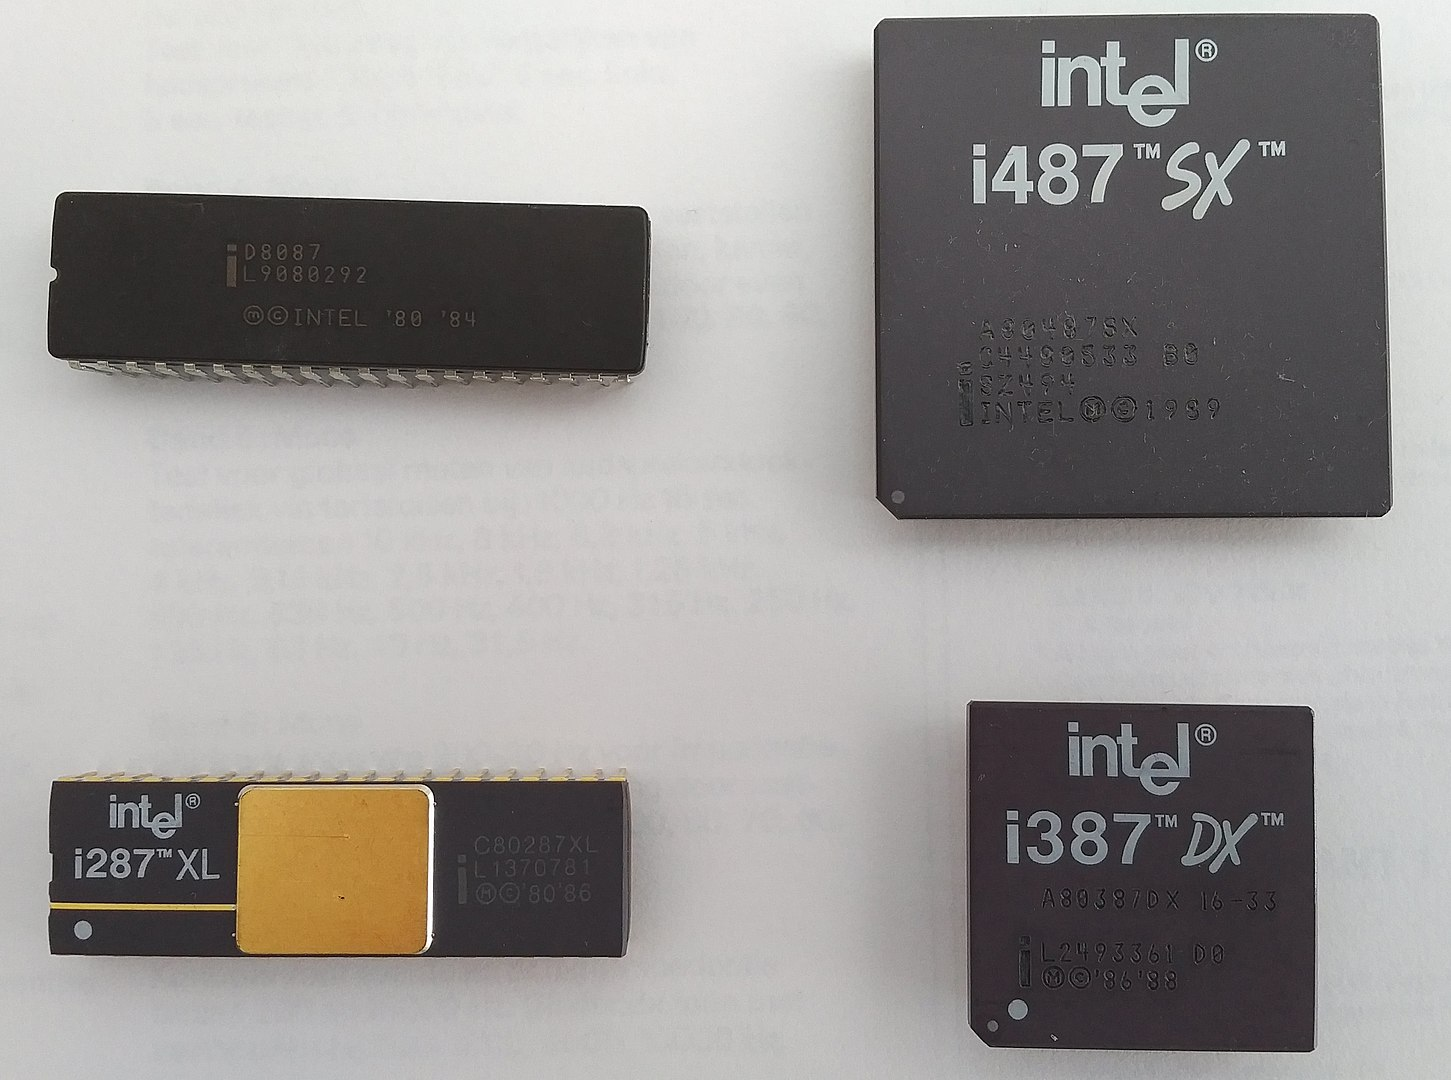
\includegraphics[width=\linewidth]{images/cpu_fpu.jpg}
                \caption{À l'origine, les FPU pouvaient être achetées séparément des processeurs.}
                \label{pic_cpu_fpu}
            \end{subfigure}
            ~ %add desired spacing between images, e. g. ~, \quad, \qquad, \hfill etc. 
              %(or a blank line to force the subfigure onto a new line)
            \begin{subfigure}[b]{0.45\linewidth}
                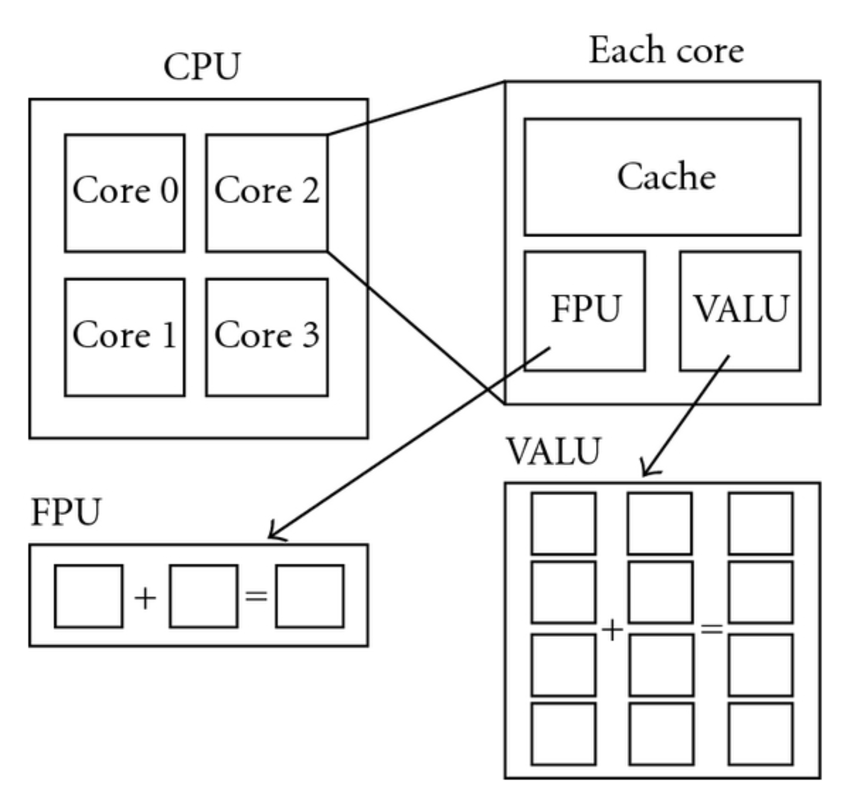
\includegraphics[width=\linewidth]{images/cpu_fpu_recent.png}
                \caption{Aujourd'hui, la FPU fait partie de chaque coeur du processeur.}
                \label{pic_cpu_fpu_recent}
            \end{subfigure}
            \caption{La FPU d'un processeur est un matériel permettant d'exécuter efficacement des instructions de calculs arithmétiques sur des nombres à virgule flottante: addition, soustraction, multiplication, division, racine carrée, etc...\protect\footnotemark }\label{fig:fpu_evo_before_after}
        \end{figure}
        \footnotetext{Source images: \url{https://en.wikipedia.org/wiki/Floating-point_unit} et \url{https://www.extremetech.com/computing/263963-intel-reverses-declares-skylake-x-cpus-two-avx-512-units}}
        
        L'ajout de la FPU directement sur les coeurs a notamment permis de réduire les latences d'accès. De plus, avec l'apparition de plateformes multiprocesseurs, la gestion d'erreurs et d'exceptions liées aux FPU externes était devenue très difficile. Le premier processeur Intel à posséder une FPU et une ALU sur la même puce est le processeur Intel 80486DX produit en 1989.  Aujourd'hui, les FPU sont des composants de haute performance capable d'exécuter plusieurs instructions de calcul sur des nombres réels grâce à des instructions vectorielles.  

        
        
        Les applications de HPC réalisent majoritairement des calculs sur nombres à virgule flottante qui sont exécutés par les FPU. Ces unités sont très sollicitées et il est important d'en connaître les caractéristiques: débit, latence, fréquence maximale soutenable par le processeur. Les instructions vectorielles les plus longues utilisent une plus grande quantité de transistors pour être exécutées. Ainsi, la chaleur émise par le processeur varie et les instructions les plus complexes ne peuvent pas être exécutées aux fréquences maximales du processeur. Les différentes fréquences atteignables pour un type d'instruction peuvent être difficiles à prévoir.
        
        %Les modèles tels que celui du \textit{roof line} (voir \autoref{sec:roofline}), ont besoin de ces caractéristiques pour pouvoir comparer la performance mesurée d'une application à celle théoriquement atteignable. 
       
       
    \subsubsection{Objectifs}
    %%%%%%%%%%%%%
    \textbf{todo revoir les objectifs a la fin}
    
        Dans la suite de cette section, nous présentons  un outil permettant de caractériser finement les performances des unités de calcul en virgule flottante (\gls{FPU}). Le développement de cet outil a été motivé par la nécessité d'obtenir différentes caractéristiques de la microarchitecture:
        \begin{enumerate}
            \item La première caractéristique pouvant être mesurée est la performance maximale atteignable par la FPU pour un certain type d'instruction. Cette performance est mesurée en nombre \gls{FLOPS} et notée \gls{flopsmax}). Elle doit être mesurée pour des types et des tailles d'instructions vectorielles différents. L'avantage de cette unité est de rendre les résultats du  \verb=Kernel Generator= comparable avec ceux d'autres benchmarks (tel que \textit{HPL} \cite{Dongarra2003}).
            
            \item La deuxième caractéristique mesurable est la latence des instructions. Il peut être intéressant de connaître celle-ci lors de l'exécution d'instructions dépendantes.
            
            \item D'autres comportements doivent être caractérisés pour anticiper et comprendre la performance de certaines applications. Parmi eux, celui de l'unité d'exécution dans le désordre. Certains codes comportant beaucoup de dépendances sont limités par la faculté du processeur à exécuter plusieurs chaînes de dépendances. 
        
        \end{enumerate}
 
        
\subsection{Kernel Generator}    
%%%%%%%%%%%%%%%%%%%%%%%%%%%%%%%%%%%%%%%%%%%%%%%%%%%%%

        Afin de répondre aux objectifs fixés dans la section précédente, nous avons développé l'outil \verb=Kernel Generator=. Il permet de générer des \gls{kernel} en assembleur pour caractériser finement le comportement des \gls{FPU}. Cet outil vise plus particulièrement les développeurs d'application dont la performance est limitée par le débit d'exécution d'instructions de calcul (\gls{computebound}). Bien que la performance des processeurs soit souvent limitée par la bande passante mémoire, une partie significative des codes est purement \gls{computebound}. 
        
        L'outil du \verb=Kernel Generator= permet de mesurer certaines caractéristiques de la FPU d'un processeur grâce à l'exécution d'un kernel généré en assembleur comportant des instructions de calcul arithmétique. Les instructions utilisées peuvent être scalaires ou vectorielles. La version actuelle de l'outil supporte les instructions de types scalaire, SSE, AVX2 et AVX512. 
            
        Grâce à ses différentes options, l'utilisateur peut générer des kernels d'instructions de types et de tailles différents. La valeur de l'outil vient de son utilisation et des différents tests que le programmeur peut réaliser. L'outil peut aussi être utilisé pour détecter des problèmes de la microarchitecture lors de l'exécution intensive d'instructions de calculs. Détecter ces comportements cachés peut ensuite permettre de mieux apprécier la performance d'une application réelle. 
            

        
        

    \subsubsection{Concept}
    %%%%%%%%%%%%%%%%%%%%%%
        L'outil \verb=Kernel Generator= est un générateur de code assembleur permettant de mesurer la performance de la FPU d'un coeur de processeur. Pour cela, l'outil génère automatiquement un programme en langage C++ contenant:
        \begin{itemize}
            \item Les instructions assembleurs sélectionnées par l'utilisateur. 
            \item Le code responsable de l'exécution et des différentes mesures de performance
        \end{itemize}
                    \begin{figure}
            \center
            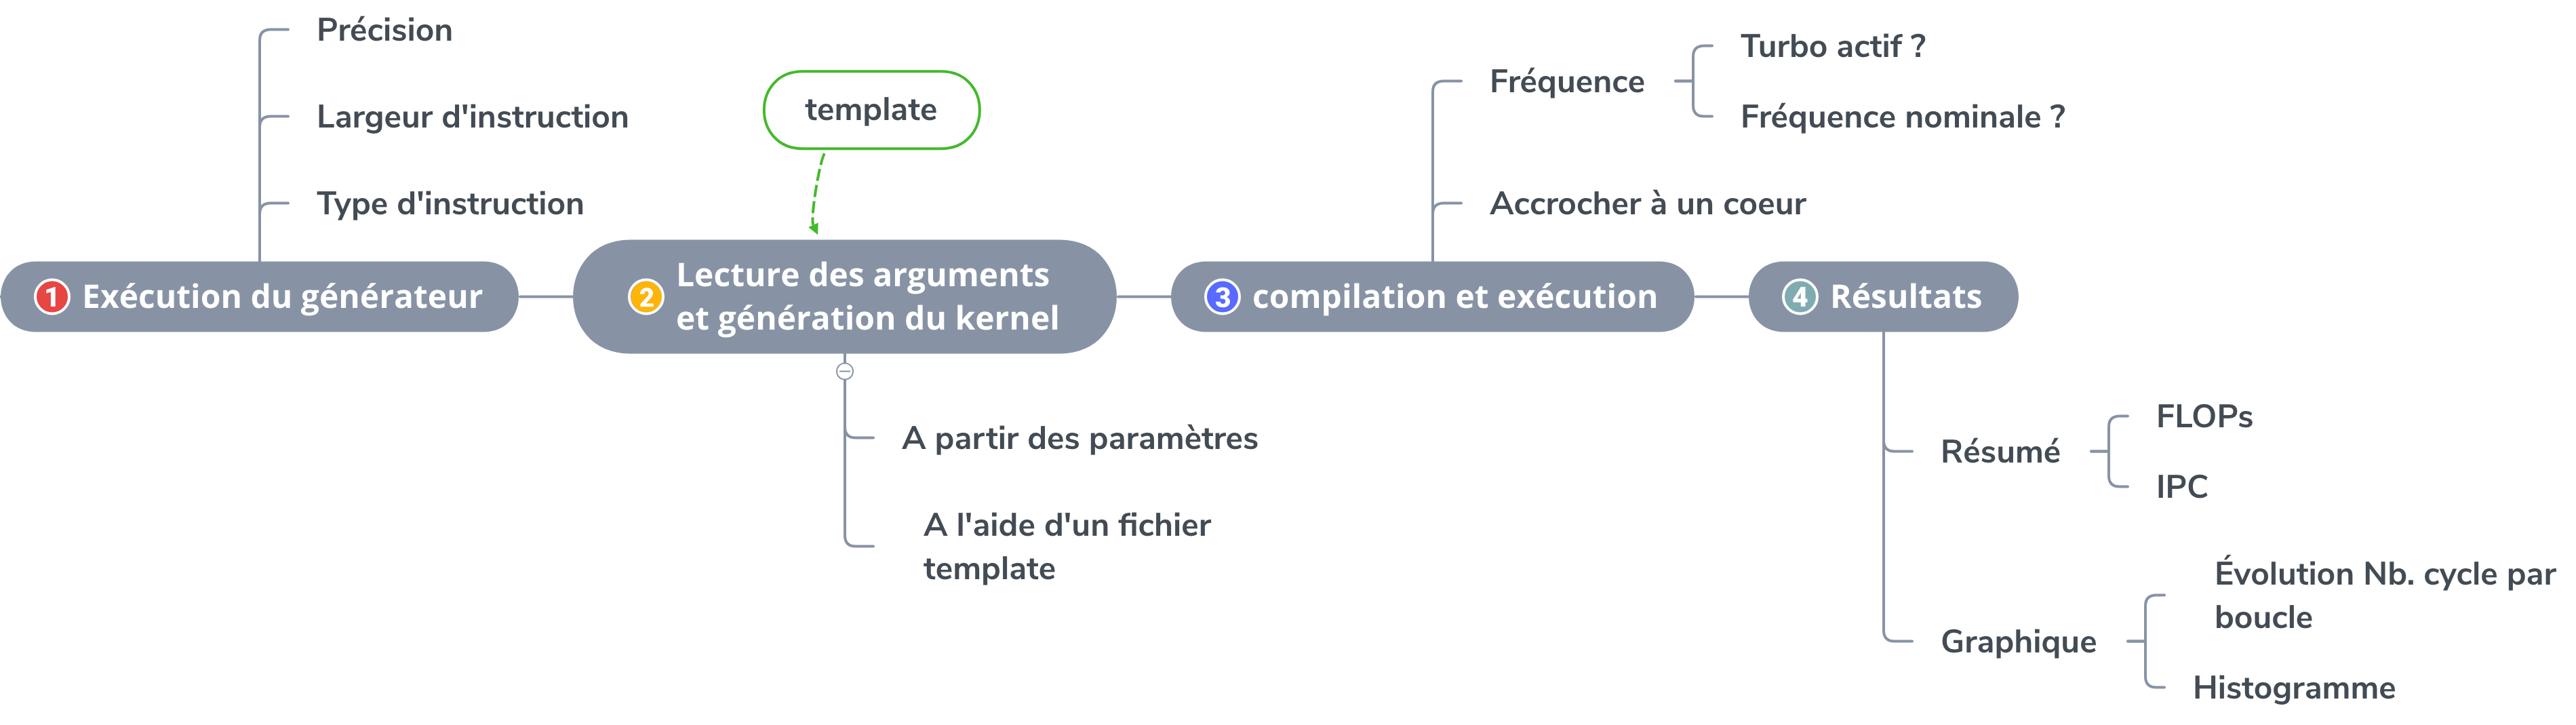
\includegraphics[width=17cm]{images/kg_workflow.png}
            \caption{\label{pic_kg_workflow} Déroulement de l'exécution du \texttt{Kernel Generator}.}
            \end{figure}
            \textbf{TODO police plus grande plus légende figure: revoir nom première étape}
            
        La \autoref{pic_kg_workflow} montre les étapes principales de l'utilisation du \verb|Kernel Generator|. Le code généré par l'outil reste simple afin de faciliter l'établissement de conclusions par utilisateur. En effet, produire un code trop complexe rendrait l'analyse des résultats trop difficile sur des  architectures aussi complexes que celles étudiées. Un exemple d'utilisation de l'outil peut être réalisé grâce à la commande suivante:\\
        \verb|./kg   -P double -W 128  -O aamm|\\
        Cette commande permet de générer un kernel de calculs utilisant quatre instructions vectorielles de 128 bits sur des nombres flottants en double précision. Le kernel généré est présenté dans l'\autoref{code_kg_exemple}. Il est composé de quatre instructions: deux additions et deux multiplications.
        
\begin{minipage}{0.97\linewidth}
\begin{lstlisting}[label=code_kg_exemple ,language=, caption=Exemple de kernel généré à l'aide de la commande \texttt{./kg   -P double -W 128  -O aamm} contenant 4 instructions vectorielles de 128 bits.]
"vaddpd %%xmm0, %%xmm1, %%xmm2;"
"vaddpd %%xmm0, %%xmm1, %%xmm3;"
"vmulpd %%xmm0, %%xmm1, %%xmm4;"
"vmulpd %%xmm0, %%xmm1, %%xmm5;"
\end{lstlisting} 
\end{minipage}

        À partir des arguments, le générateur écrit un programme en langage C++ qu'il compile et exécute. Les résultats sont ensuite présentés sous forme de texte dans le terminal ou sous forme de graphique (nécessite Python).
        Le choix du langage assembleur a été motivé par la volonté de s'assurer que les instructions générées étaient bien exécutées. En effet, les compilateurs deviennent toujours plus performants et optimisent les codes rendant l'analyse de performance plus difficile. De plus, ils peuvent détecter l'artificialité d'un code et contourner son exécution. En générant nous même le code assembleur, nous nous assurons que la performance du code mesuré est bien celle du code attendu.
    
       
    \subsubsection{Les options.}\label{sec:kg_option} 
    
        Une des forces du \verb|Kernel Generator| vient de sa capacité à générer un grand nombre de benchmarks différents. Ceci est possible grâce à l'utilisation des différentes options dont les principales sont listées ci-dessous:
    
        \paragraph{\texttt{-{}-operation [a,m,f]+}} Lister les opérations à réaliser par le kernel à l'aide d'une chaîne de caractères composé des lettres \texttt{a}, \texttt{m} et \texttt{f} correspondant aux opérations suivantes : addition (a), multiplication (m) ou \gls{FMA} (f). Différentes opérations peuvent être mixées et seront insérées dans le \gls{kernel} dans le même ordre. Un script externe peut alors être utilisé pour générer des kernels testant différentes combinaisons d'opérations. En faisant varier à la fois les opérations et la taille des instructions, l'outil permet de découvrir des comportements cachés des architectures.

        \paragraph{\texttt{-{}-precision (single | double)}} Définir la précision utilisée pour réaliser les calculs: simple ou double. Pour le moment, des instructions ayant des précisions différentes ne peuvent pas être mélangées dans un même kernel.
        
        \paragraph{\texttt{-{}-width (64 | 128 | 256 | 512)}} Définir la \textit{largeur} des instructions vectorielles utilisées. Sur une architecture Intel, ces instructions correspondents aux ISA suivantes: MMX (64), SSE (128), AVX (256) et AVX-512 (512). Pour le moment, des instructions vectorielles de tailles  différentes ne peuvent pas être mixées dans un même kernel.
        
        \paragraph{\texttt{-{}-dependency N}} Générer une instruction  dont un opérande est le résultat produit par l'instruction précédente. Un nombre \texttt{N} peut être donné pour générer plusieurs chaînes de dépendances. Cette option est particulièrement utile pour mesurer la latence des instructions et la performance du tampon d'exécution dans le désordre.
        
        \paragraph{\texttt{-{}-binding N}} Accrocher (\textit{bind}) le benchmark généré à un coeur spécifique. Le benchmark n'étant pas parallélisé, il est nécessaire d'en exécuter plusieurs versions en parallèle pour tester la performance d'un processeur lorsque plusieurs coeurs sont utilisés. Les différents processus crées peuvent alors être \textit{accrochés} aux différents coeurs du processeur à l'aide d'un script externe.
        
        \paragraph{\texttt{-{}-unroll N}} Appliquer l'optimisation du déroulement de boucle \texttt{N} fois. Cette optimisation permet de dérouler plusieurs fois le corps de la boucle à l'intérieur de celle-ci pour réduire l'impact du traitement des instructions de contrôle de la boucle (incrémentation et comparaison) sur les performances du benchmark. 
        
        \paragraph{\texttt{-{}-frequency (true | false)}} Générer puis exécuter une fonction en début de benchmark qui mesure la fréquence du processeur. Les calculs des résultats sont impactés par l'utilisation du mode turbo. En connaissant la valeur de la fréquence turbo, ces résultats peuvent être ajustés. En effet, la mesure de la performance du benchmark est réalisée en utilisant la valeur de la fréquence de base du processeur. 
        
        \paragraph{\texttt{-{}-loopsize N}} Améliorer la précision des résultats et éliminer les potentiels bruits de mesure en réalisant \texttt{N} mesures.
    
    
    \subsubsection{Fonctionnement du générateur}
    %%%%%%%%%%%%%%%%%%%%%%
        
        Une fois les différentes options analysées, le générateur va écrire un programme C++ contenant le benchmark à exécuter. Tous les benchmarks ont une partie commune de code qui est stockée dans un fichier \textit{template}. Le générateur s'occupe seulement d'écrire la partie en assembleur dans ce fichier et d'initialiser quelques variables (nombre de mesures, coeur sur lequel s'exécuter). Le \textit{template} contient le code permettant de mesurer les résultats, de calculer la fréquence et d'afficher le résultat  dans le terminal. Un exemple d'exécution du générateur est résumé sur la \autoref{pic_kg_generation}. 

        \begin{figure}[h!]
            \center
            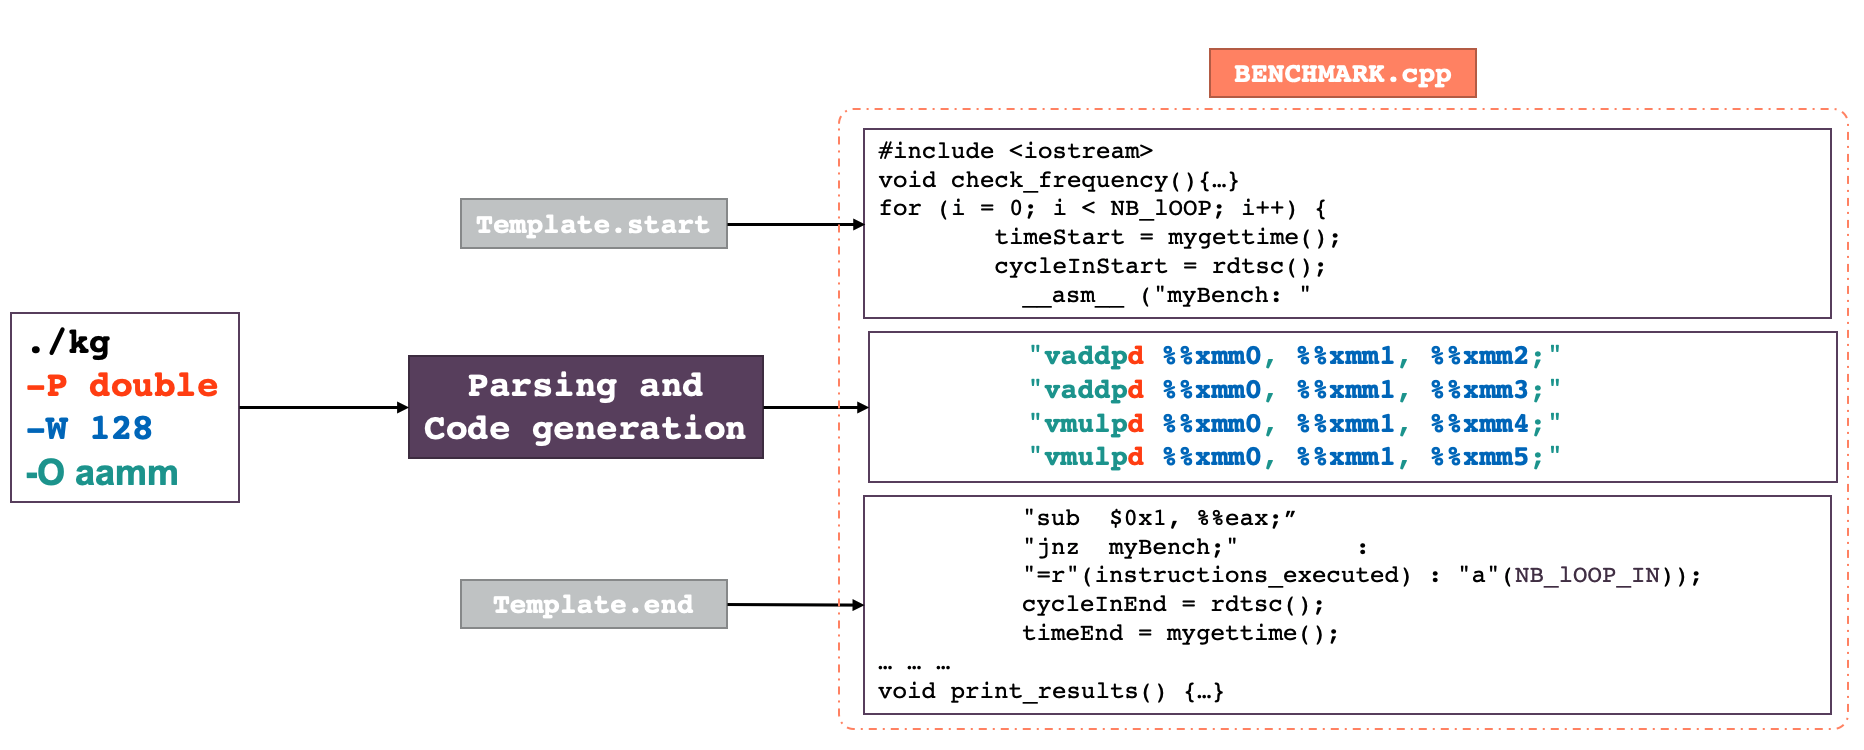
\includegraphics[width=16cm]{images/kg_generation.png}
            \caption{\label{pic_kg_generation}Génération du benchmark à partir de la ligne de commande entrée par l'utilisateur. La partie commune du code est stockée dans un fichier de \textit{template}.}
        \end{figure}
        
        Lorsque le code du benchmark généré, celui-ci est compilé automatiquement par le générateur (le compilateur utilisé peut facilement être modifié). Le fichier source et l'exécutable sont créés dans le dossier courant de l'utilisateur. L'exécutable peut ensuite être utilisé sans passer de nouveau par le générateur. Un exemple de résultat de l'exécution du benchmark est présenté dans l'\autoref{output:basic_gflops}.
    
 \begin{minipage}{0.97\linewidth}
 \begin{lstlisting}[label=output:basic_gflops ,language=, caption=Exemple d'exécution d'un benchmark de quatre instructions AVX-512.]
./kg -W 512 -O aamm -P double -U 4 -S 30000 -L 500000

--------------------  CHECK FREQUENCY  ------------------------
+ Base      frequency is 2.69GHz
+ Current   frequency is 2.68GHz
+ OK: the core is running at his frequency based value

------------------  INSTRUCTIONS SUMMARY -----------------------
_label_|   NB INSTRUCTIONS      Time    FREQUENCY   Giga_inst/sec     IPC
_value_|      240000000000      44.7         2.69            5.37    1.99

----------------------  FLOP SUMMARY  --------------------------
 PRECISION     FLOP/cycle         FLOP/second
    Single              0                   0
    Double             16             4.3e+10
----------------------------------------------------------------


\end{lstlisting}   
 \end{minipage}   
        Le benchmark généré comporte quatre instructions vectorielles AVX-512: deux additions et deux multiplications. Le processeur utilisé est un  Intel Xeon 6150 cadencé à 2.70GHz. Pour cette expérimentation, la fréquence turbo a été désactivée. Pour améliorer la précision des résultats, la boucle générée est déroulée 4 fois. La boucle réalise 500 000 itérations et sa performance est mesurée 30 000 fois. Le CPU est capable d'exécuter deux opérations flottantes vectorielles par cycle d'horloge. Pour des données en doubles précisions, cela correspond à réaliser 16 opérations flottantes par cycle. La puissance de calcul atteinte par l'exécution du benchmark sur un coeur est de 43 GFLOPS. Pour chaque mesure le nombre de cycles et le temps nécessaire à l'exécution de la boucle sont sauvegardés dans un fichier. Ce fichier peut ensuite être affiché avec un script python (voir \autoref{fig:kg_graph}). La \autoref{pic_kg_plot} permet de voir comment la performance du benchmark évolue au fil des exécutions. On peut détecter des problèmes de détérioration des performances pouvant être dus à un mauvais refroidissement du processeur par exemple.  La \autoref{pic_kg_hist} affiche l'histogramme permettant de voir deux familles de performance. Dans cet exemple, la différence entre ces deux familles est inférieure à 0,02\%. Il peut cependant arriver que pour certaines architectures, le processeur ne soit pas capable de maintenir une performance constante lors de l'exécution de certaines instructions. Ce comportement pourra alors être mis en évidence grâce à ce graphique (\autoref{pic_kg_hist}).
        
        \begin{figure}
            \centering
            \begin{subfigure}[b]{0.45\linewidth}
                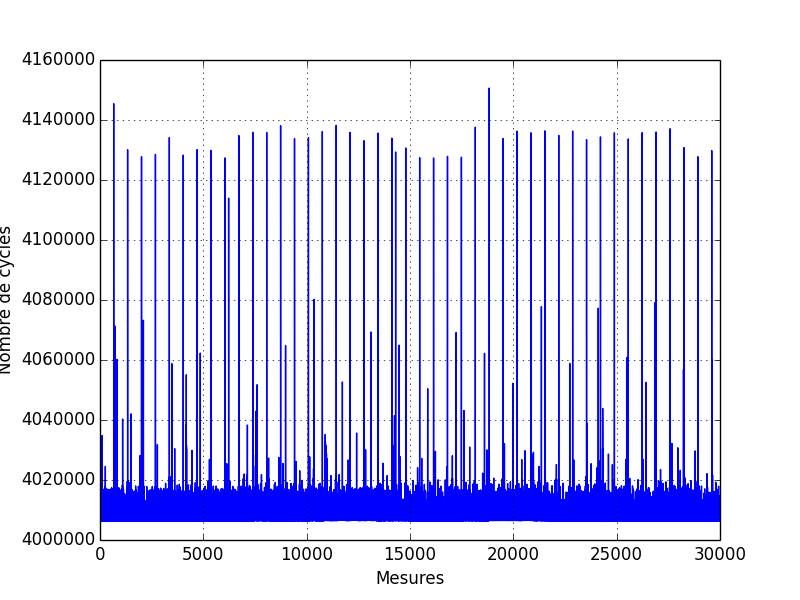
\includegraphics[width=\linewidth]{images/kg_plot.png}
                \caption{Évolution du nombre de cycles nécessaires pour l'exécution de la boucle de benchmark}
                \label{pic_kg_plot}
            \end{subfigure}
            ~ %add desired spacing between images, e. g. ~, \quad, \qquad, \hfill etc. 
              %(or a blank line to force the subfigure onto a new line)
            \begin{subfigure}[b]{0.45\linewidth}
                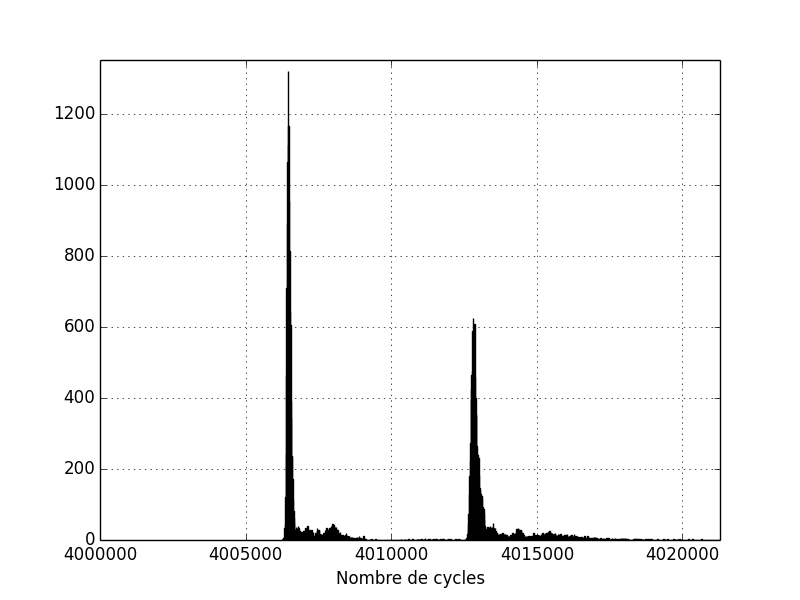
\includegraphics[width=\linewidth]{images/kg_hist.png}
                \caption{Histogramme du nombre de cycles nécessaires}
                \label{pic_kg_hist}
            \end{subfigure}
            \caption{Grâce à un script python, le fichier de résultat peut être affiché sous forme de graphiques. }\label{fig:kg_graph}
        \end{figure}
    
  
        %%%% OPTION %%%    
    
    
    \subsubsection{Validation des résultats}
    
        Lors du développement du générateur, il a été nécessaire d'utiliser des outils nous permettant de valider les performances rapportées par le benchmark. Pour s'assurer du bon fonctionnement du benchmark sur de nouvelles architectures, certaines de ces méthodes de vérification ont été implémentées dans l'outil directement. 
        
        %#TODO enelver le compteur je pense qu'il est NDA pour HPE
        \paragraph{Validation du nombre d'instructions.} 
            
            La première valeur à valider est de s'assurer que le bon nombre d'instructions a été exécuté par le benchmark. Le benchmark affiche le nombre d'instructions qui devrait être exécuté. Un moyen de le vérifier est d'utiliser les compteurs matériels. L'outil \verb|perf| permet de mesurer le nombre d'évènements d'un compteur en utilisant son adresse. La ligne de commande suivante permet de compter les opérations flottantes réalisées par le benchmark: \verb|perf stat -e /rffc7 ./benchmark|. Le résultat du benchmark ci-dessus prévoyait l'exécution de 240,000,000,000 opérations. La commande \verb|perf stat| retourne une valeur de 240,000,210,024 opérations (une instruction FMA compte pour deux). Pour comprendre d'où proviennent les instructions supplémentaires, nous avons mesuré différentes versions du benchmark avec différentes longueurs de boucle (5000, 10000 et 20000). Le \autoref{tab:kg_vs_perf} donne les résultats affichés par le benchmark et par la commande précédente utilisant l'outil \verb|perf|. Les résultats de \verb|perf| mesurent le bon nombre d'instructions avec 2124 opérations supplémentaires à chaque fois. Ces instructions supplémentaires correspondent au traitement des résultats.
    
            \begin{table}[h!]
            \centering
            %\resizebox{\textwidth}{!}{%
            \begin{tabular}{@{}lcc@{}}
            \toprule
             Commande utilisée & Nombre d'instructions attendu & Résultat perf \\ \midrule
            ./kg -W 512 -O aamm -S 300 -L 5000 & 6000000 & 6002124 \\
            ./kg -W 512 -O aamm -S 300 -L 10000 & 12000000 & 12002124 \\
            ./kg -W 512 -O aamm -S 300 -L 20000 & 24000000 & 24002124 \\ \bottomrule
            \end{tabular}%
            %}
            \caption{Vérification du nombre d'instructions exécutées avec l'outil \texttt{perf}.}
            \label{tab:kg_vs_perf}
            \end{table}
        
        
        \paragraph{Validation de l'IPC.} 
        
            La validation du nombre d'\gls{IPC} du processeur peut elle aussi être réalisée grâce à \verb|perf|: \verb|perf stat ./benchmark|. Pour générer le benchmark la commande suivante a été utilisée:\\
            \verb|./kg -W 512 -O aamm -P double -S 1000 -L 90000000|\\
            Lors de son exécution, le benchmark donne un IPC de 2 alors que la commande \verb|perf| donne un résultat de 3. Cette différence peut être expliquée en regardant le code assembleur généré (voir \autoref{lst:kg:ipc}).
        
\begin{minipage}{0.965\linewidth}
        \begin{lstlisting}[label=lst:kg:ipc ,language=C, caption={Code généré par la commande ./kg -W 512 -O aamm -P double. Le benchmark mesure la performance de la boucle à l'aide du compteur de cycle (\texttt{rdtsc()}). Cette mesure comprend l'exécution des instructions de calculs du kernel mais aussi les deux instructions de la gestion de boucle \texttt{sub} et \texttt{jnz}.}]
cycleInStart = rdtsc();
__asm__ ("" 
    "myBench: " 
		"vaddpd %%zmm0, %%zmm1, %%zmm2; "
		"vaddpd %%zmm0, %%zmm1, %%zmm3; "
		"vmulpd %%zmm0, %%zmm1, %%zmm4; "
		"vmulpd %%zmm0, %%zmm1, %%zmm5; "
    "sub  $0x1, %%eax;"
    "jnz  myBench;"		: "=r" (instructions_executed) : "a" (NB_lOOP_IN));
cycleInEnd = rdtsc();
\end{lstlisting}
\end{minipage}\\
            Le résultat donné par le benchmark ne prend en considération que les quatre instructions de calculs pour calculer l'IPC alors que l'outil \verb|perf| compte la totalité des instructions exécutées. Notre calcul prend pour postulat que les deux instructions de gestion de boucle (la décrémentation \verb|sub|, et le saut conditionnel \verb|jnz|) ne rentre pas dans le profil de l'exécution. En effet, grâce au prédicateur de branchement, l'instruction de saut peut effectivement être enlevée de nos calculs. 

            Concernant la soustraction, nous avons réalisé un test pour vérifier l'impact de soustraction de nombre entier lors de l'exécution d'un code ne réalisant que des opérations sur des nombres flottants (voir \autoref{code:sub}). En mesurant la performance de ce code, nous avons observé que 4 soustractions sur des nombres entiers n'impactent pas la performance de la boucle. Au-delà de 4, le processeur a besoin de cycles supplémentaires pour les exécuter. Ainsi les deux instructions de gestion de boucles peuvent être ignorées dans le calcul. Pour réduire l'impact de ces deux instructions sur le résultat donnée par \verb|perf|, nous avons implémenté une option de déroulement de boucle (\textit{unrolling}). En utilisant l'option \verb|-U 10|, le benchmark généré déroule la boucle 10 fois permettant de réduire l'impact des instructions de la gestion de boucle (incrémentation et test). Grâce à cette option, nous avons pu valider l'IPC calculé par notre benchmark avec celui mesuré par \verb|perf| (2 instructions par cycle).
        
            \begin{minipage}{0.965\linewidth}         \begin{lstlisting}[label=code:sub ,language=C, caption={En ajoutant jusqu'à 3 soustractions, nous avons pu vérifier que la soustraction utilisée pour la gestion de la boucle n'avait aucun impact sur la performance du benchmark. En effet, la soustraction sur un nombre entier n'utilise pas la FPU.}]
cycleInStart = rdtsc();
__asm__ ("" 
    "myBench: " 
       "vaddpd %%zmm0, %%zmm1, %%zmm2; "
       "vaddpd %%zmm0, %%zmm1, %%zmm3; "
       "vmulpd %%zmm0, %%zmm1, %%zmm4; "
       "vmulpd %%zmm0, %%zmm1, %%zmm5; "
       "sub  $0x1, %%ebx;" //soustraction artificielle
       "sub  $0x1, %%ebx;" //soustraction artificielle
       "sub  $0x1, %%ebx;" //soustraction artificielle
    "sub  $0x1, %%eax;"
    "jnz  myBench;"		: "=r" (instructions_executed) : "a" (NB_lOOP_IN));
cycleInEnd = rdtsc();
\end{lstlisting} \end{minipage}
        
        
        \paragraph{Validation des FLOPS.} 
            Afin de valider le nombre de calculs réalisés, deux méthodes ont été employées.
            La première méthode consiste à utiliser d'un outil développé en interne appelé \verb=mygflops=. Cet outil affiche le nombre d'opérations exécutées en consultant les compteurs matériels de chaque coeur. Le résultat sépare les différentes tailles d'instructions vectorielles utilisées. La commande, le résultat du benchmark et celui de \verb=mygflops= sont présentés dans l'\autoref{lst:basic_gflops}. 
        
\begin{minipage}{0.97\linewidth}         \begin{lstlisting}[label=lst:basic_gflops ,language=C, caption={L'utilisation de l'outil \texttt{mygflops}, développé par notre équipe, a permis de valider les résultats donnés par notre benchmark (\textit{ligne 6}). L'outil \texttt{mygflops} utilise les compteurs matériels pour mesurer les différentes instructions de calculs réalisées et permet de valider nos résultats (\textit{ligne 19}).}]
./kg -W 128 -O aamm -P double -U 10 -S 10 -L 90000000
...
----------------------  FLOP SUMMARY  --------------------------
 PRECISION     FLOP/cycle         FLOP/second
    Single              0                   0
    Double           4.00            1.06e+10
----------------------------------------------------------------
...

********************** MYGFLOPS ***********************
     
Single-precision SSE/AVX :            0.000000 GFlop/s --  0.0% of Flops

       0.0%  32-bit SSE/AVX instructions (0.0%)
       0.0% 128-bit SSE/AVX instructions (0.0%)
       0.0% 256-bit AVX instructions     (0.0%)
       0.0% 512-bit AVX instructions     (0.0%)
     
Double-precision SSE/AVX :            10.572521 GFlop/s -- 100.0% of Flops

       0.0%  64-bit SSE/AVX instructions (  0.0%)
     100.0% 128-bit SSE/AVX instructions (100.0%)
       0.0% 256-bit AVX instructions     (  0.0%)
       0.0% 512-bit AVX instructions     (  0.0%)

\end{lstlisting} \end{minipage}
        
        Malheureusement, l'outil \verb=mygflops= n'est pas disponible en accès libre pour le reste de la communauté. Nous avons ainsi développé une méthode de validation des résultats interne au benchmark. En fonction des opérations utilisées, les registres sont initialisés avec différentes valeurs significatives. Par exemple, pour vérifier que le bon nombre d'additions a été exécuté, les registres sont initialisés à la valeur 1. À la fin du benchmark, les registres ayant participé au benchmark sont sommés pour vérifier que le bon nombre d'additions a été exécuté. Grâce à cette méthode, nous avons la certitude que les opérations sont réellement exécutées par le processeur et qu'aucune optimisation lui permettant d'en éviter n'est possible ou une erreur de logique.
        

    \subsubsection{Mesure de la fréquence}
    %%%%%%%%%%%%%%%%%%%%%%
        Plus un processeur utilise une fréquence élevée, plus sa consommation électrique est élevée. Pour cette raison, Intel a adopté différents niveaux de fréquences pour ses processeurs. Cela permet d'augmenter les performances en cas de besoin et de limiter la consommation d'énergie si le processeur n'a pas besoin d'être pleinement utilisé. Les instructions les plus complexes (instructions vectorielles) nécessite l'utilisation de plus de transistors que les instructions scalaires. L'énergie dissipée est alors plus élevée, empêchant le processeur d'utiliser sa fréquence maximale pour l'exécution de telles instructions (voir \autoref{fig:cpu_freq_avx}). 
        
        \begin{figure}
            \center
            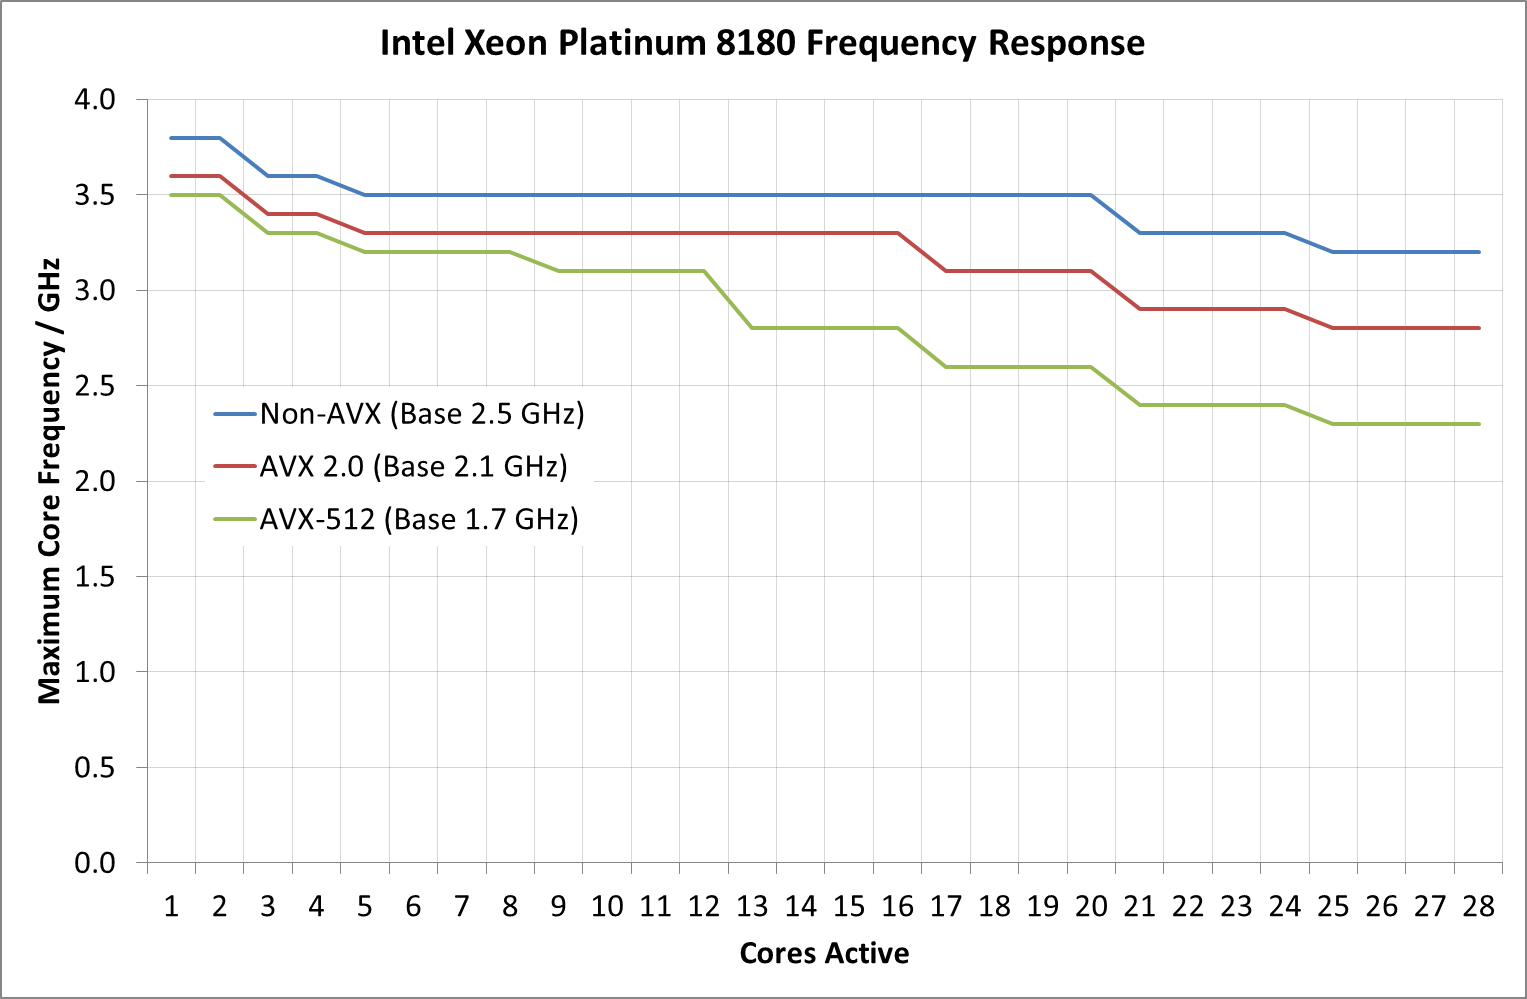
\includegraphics[width=10cm]{images/cpu_freq_avx.png}
            \caption{\label{fig:cpu_freq_avx} La fréquence soutenable par le processeur (axe des ordonnées) varie en fonction du nombre de coeur utilisés (axes des abscisses) et du type d'instructions exécutées: scalaire (en bleu), AVX 2.0 (en rouge) ou AVX 512 (en vert)\protect\footnotemark.}
        \end{figure}
        \footnotetext{Source du graphique: 
        \href{https://www.anandtech.com/show/11544/intel-skylake-ep-vs-amd-epyc-7000-cpu-battle-of-the-decade/8}{\nolinkurl{https://www.anandtech.com/show/11544/intel-skylake-ep-vs-amd-epyc}}
        }
        
        
        L'instruction \verb|rdtsc| est utilisée pour lire le compteur matériel mesurant le nombre de \textit{tics} de l'horloge depuis la dernière réinitialisation du processeur \cite{code:rdtsc}. La fréquence à laquelle ce compteur est incrémenté ne varie pas et correspond à la \textit{fréquence de base nominale} du processeur. Cette fréquence est indépendante de la fréquence d'horloge réelle, qui peut varier. Si les fréquences des processeurs devaient varier, les mesures effectuées avec \verb|rdtsc| seraient erronées. C'est pourquoi nous conseillons de fixer la fréquence du processeur avant l'exécution du micro-benchmark. Dans le cas d'une fréquence fixe différente de la fréquence de base nominale, nous avons mis en place une vérification qui calculera ensuite cette fréquence, et ajustera les résultats mesurés par \verb|rdtsc| comme le calcul de l'\gls{IPC}. Cette fonctionnalité de vérification de la fréquence et de la correction de résultat est utilisable avec l'option \verb|-F true|. Afin d'apporter les corrections voulues, nous avons besoin de mesurer la fréquence de base du processeur ainsi que la fréquence utilisée pour l'exécution.
        
        \paragraph{Mesurer la fréquence de base.} Nous avons développé un code permettant de mesurer la fréquence de base. Il utilise la fonction \verb=sleep()= qui attend un certain nombre de microsecondes, ainsi que l'instruction \verb|rdtsc|. Ainsi nous pouvons calculer la fréquence avec le rapport $cycleSpent / timeSpent$ comme indiqué sur l'\autoref{code:base_freq}. 
        

\begin{minipage}{0.97\linewidth}         \begin{lstlisting}[label=code:base_freq ,language=C, caption={Code utilisé pour mesurer la fréquence de base du processeur. La fonction \texttt{mygettime()} utilise la fonction \texttt{gettimeofday()}\protect\footnotemark ~permet de mesurer le temps nécessaire à l'exécution du code.}]
timeStart = mygettime();
cycleInStart = rdtsc();
    usleep(10000);
cycleInEnd = rdtsc();
timeEnd = mygettime();
cycleSpent = (cycleInEnd - cycleInStart);
freq_Base = cycleSpent / (1000000000 * (timeEnd - timeStart));
\end{lstlisting} \end{minipage}
\footnotetext{gettimeofday(2) - \url{http://man7.org/linux/man-pages/man2/gettimeofday.2.html}}
\textbf{todo forme extrait des centres: la légende est trop collées au truc gris}

        \paragraph{Mesurer la fréquence réelle.} Pour pouvoir ajuster les résultats affichés par le benchmark, il est nécessaire de connaître la fréquence à laquelle le processeur est capable de fonctionner. Cette fréquence peut varier soit avec l'utilisation du mode \textit{turbo} soit en limitant la fréquence de façon logicielle. Pour réaliser cette mesure, nous sommes partis du constat que tous les processeurs modernes sont capables d'exécuter une soustraction sur un registre par cycle d'horloge. 
        
         
\begin{minipage}{0.97\linewidth}         \begin{lstlisting}[label=code:cur_freq ,language=C, caption={Code utilisé pour mesurer la fréquence réelle du processeur.}]
cycleInStart = rdtsc();
__asm__ ("aloop: "
    "sub $0x1,%%eax;"
    "sub $0x1,%%eax;"
    "sub $0x1,%%eax;"
    "sub $0x1,%%eax;"
    "jnz aloop" : : "a" (80000000UL)
);
cycleInEnd = rdtsc();
cycleSpent = (cycleInEnd - cycleInStart);
\end{lstlisting} \end{minipage}  
        
        Dans l'\autoref{code:cur_freq}, le registre \verb|%eax| est initialisé à \verb|80000000|. Grâce à notre hypothèse, il est possible de prévoir que le processeur réalisera ces \verb|80000000| soustractions en autant de cycles. Nous mesurons le nombre de cycles nécessaire à l'exécution du code à l'aide de l'instruction \verb=rdtsc=. Ce nombre correspond au nombre de cycle à la fréquence nominale du processeur. En faisant le rapport entre le nombre de cycles mesurés et celui attendu par notre hypothèse, il est possible de déterminer si le processeur utilise une fréquence plus ou moins rapide que sa fréquence nominale. Nous calculons ainsi l'\gls{IPC} de cette boucle en faisant le rapport $\frac{80000000}{cycleSpent}$.
        \begin{itemize}
            \item \verb|IPC == 1|: Le processeur utilise sa fréquence de base
            \item \verb|IPC < 1|: Le processeur utilise une fréquence inférieure à sa fréquence de base.
            \item \verb|IPC > 1|: Le processeur est capable d'exécuter des instructions à une fréquence plus élevée que sa fréquence de base (turbo).
        \end{itemize}
    
    
    
        \paragraph{Ajuster les résultats.} En connaissant la fréquence de base et la fréquence accessible par le processeur, les résultats donnés par le benchmark peuvent être ajustés. Nous avons utilisé un script externe pour verrouiller la fréquence du processeur Intel Xeon 6150 à 2,00 GHz. Ce processeur a une fréquence de base de 2,70 GHz. Le code présenté ci dessus nous a permis de mesurer un \gls{IPC} égal à 0,742. Cela signifie que le processeur utilise une fréquence égale à 74,2\% de sa fréquence de base, soit 2,00 GHz. Ce dernier test nous a permis de valider la méthodologie basée sur \verb|rdtsc| pour mesurer la fréquence réelle du processeur. Ainsi, nous pouvons ajuster les résultats donnés par notre outil grâce à l'option \verb|--frequency true|.
        \textbf{todo remplacer NOMINALE par DE BASE}

    
\subsection{Résultats}
%%%%%%%%%%%%%%%%%%%%%%%%%%%%%%%%%%%%%%%%%%%%%%%%%%%%%
    À la suite du développement du générateur de \glspl{kernel}, plusieurs expérimentations ont pu être réalisées. Dans cette section, nous présentons les principaux résultats obtenus lors de la caractérisation de processeurs Intel Skylake.
   
   
   

    \subsubsection{Vérifier les performances théoriques}
    %%%%%%%%%%%%%%%%%%%%%%%%%%%%%%%%%%%%%%%%%%%%%%%%%%%%%
    Le \verb|Kernel Generator| peut être utilisé pour mesurer les performances maximales atteignables par un processeur. Cette performance mesurée en \gls{FLOPS} est notée \gls{flopspeak}. Pour illustrer cette utilisation, nous avons étudié les performances du processeur Intel Xeon 6150 cadencé à 2.7 GHz, possédant 18 coeurs et disposant d'un mode Turbo. Les résultats de cette expérimentation sont donnés dans le \autoref{tab:kg_vs_intel}. 
    
    Comme expliqué dans l'introduction ci-dessus, la fréquence  soutenable par un processeur dépend de la complexité des instructions exécutées et du nombre de coeurs utilisés. La performance de calcul théorique varie donc en fonction de chaque configuration \texttt{\{nombre de coeurs, type d'instructions, Turbo ON/OFF\}}. Pour permettre le calcul de \gls{flopspeak}, Intel donne dans sa documentation les différentes fréquences supportées par le processeur\footnote{\url{https://www.intel.com/content/dam/www/public/us/en/documents/specification-updates/xeon-scalable-spec-update.pdf}}. Ces valeurs sont reportées dans la 4e ligne du \autoref{tab:kg_vs_intel}. Pour un type d'instruction et un nombre de coeur donné, la performance du processeur dépend de l'activation ou non du turbo:
    \begin{itemize}
        
        
        \item \textbf{Turbo ON}: si le turbo est activé, la documentation du processeur donne la fréquence maximale atteignable par le processeur pour une configuration \texttt{\{nombre de coeurs, type d'instructions\}} donnée. Cette fréquence, appelée \textit{Maximum Core Frequency} (MCF), n'est pas garantie. Elle est seulement atteignable si la température du processeur le permet. En fonction de sa qualité de fabrication (fuite de courant) et de l'efficacité de son système de refroidissement, la fréquence maximale atteignable peut varier de 20\%.
        
        \item \textbf{Turbo OFF}: si le turbo est désactivé, la documentation donne la fréquence minimale que le processeur utilisera pour exécuter les instructions. Cette fréquence, appelée \textit{Base Core Frequency} (BCF), est dite \textit{garantie}, car le processeur n'utilisera pas de fréquence inférieure à celle-ci.  La fréquence BCF peut donc être utilisée pour calculer une limite inférieure de la performance du processeur. Si la température et la conception du processeur le permettent, le processeur peut utiliser des fréquences plus élevées. Cependant, comme le turbo est désactivé, la fréquence ne pourra pas dépasser la fréquence de base du processeur (2.7 GHz dans notre exemple).
        
    \end{itemize}
    
    
    Le but de cette expérimentation est d'utiliser le \verb|Kernel Generator| pour vérifier la fréquence atteignable par le processeur pour différentes configurations. La fréquence maximale atteignable par le processeur n'étant pas garantie (même lorsque le turbo est activé), seul l'exécution du kernel peut permettre de mesurer la performance maximale atteignable par le processeur. Cette performance, mesurée en \gls{FLOPS}, est notée \gls{flopsmax}. Pour chaque type d'instructions (Non-AVX, AVX 2.0 et AVX-512), \gls{flopsmax} peut être mesurée en exécutant des instructions \gls{FMA}. Nous avons utilisé le \verb|Kernel Generator| pour créer trois benchmarks utilisant trois tailles d'instructions (scalaire, 256 et 512 bits) avec la commande suivante:\\
\begin{minipage}{0.97\linewidth}         \begin{lstlisting}
./kg -W {64,256, 512} -O ffffffffffffff -P double -U 80 -S 1 -L 90000000
\end{lstlisting} \end{minipage}\\


    
    

    \begin{table}[h!]
    \centering
    \resizebox{\textwidth}{!}{%
    \begin{tabular}{|l|cc|cc|cc|cc|cc|cc|}
    \hline
    Jeu d'instruction & \multicolumn{4}{c|}{\cellcolor[HTML]{67FD9A}Non-AVX} & \multicolumn{4}{c|}{\cellcolor[HTML]{34FF34}AVX 2.0} & \multicolumn{4}{c|}{\cellcolor[HTML]{009901}AVX 512} \\ \hline
    Turbo & \multicolumn{2}{c|}{\cellcolor[HTML]{FFFFC7}OFF} & \multicolumn{2}{c|}{\cellcolor[HTML]{FCFF2F}ON} & \multicolumn{2}{c|}{\cellcolor[HTML]{FFFFC7}OFF} & \multicolumn{2}{c|}{\cellcolor[HTML]{FCFF2F}ON} & \multicolumn{2}{c|}{\cellcolor[HTML]{FFFFC7}OFF} & \multicolumn{2}{c|}{\cellcolor[HTML]{FCFF2F}ON} \\ \hline
    Nombre de coeurs & \multicolumn{1}{c|}{\cellcolor[HTML]{ECF4FF}1} & \cellcolor[HTML]{CBCEFB}18 & \multicolumn{1}{c|}{\cellcolor[HTML]{ECF4FF}1} & \cellcolor[HTML]{CBCEFB}18 & \multicolumn{1}{c|}{\cellcolor[HTML]{ECF4FF}1} & \cellcolor[HTML]{CBCEFB}18 & \multicolumn{1}{c|}{\cellcolor[HTML]{ECF4FF}1} & \cellcolor[HTML]{CBCEFB}18 & \multicolumn{1}{c|}{\cellcolor[HTML]{ECF4FF}1} & \cellcolor[HTML]{CBCEFB}18 & \multicolumn{1}{c|}{\cellcolor[HTML]{ECF4FF}1} & \cellcolor[HTML]{CBCEFB}18 \\ \hline
    \rowcolor[HTML]{EFEFEF} 
    Fréquence (GHz) (source Intel) & 2.7 & 2.7 & 3.7 & 3.4 & 2.3 & 2.3 & 3.6 & 3.0 & 1.9 & 1.9 & 3.5 & 2.5 \\ \cline{1-1}
    \rowcolor[HTML]{EFEFEF} 
    \gls{flopspeak} (GFLOPS) & 10.8 & 194.4 & 14.8 & 244.8 & 36.8 & 662.4 & 57.6 & 864 & 60.8 & 1094 & 112 & 1440 \\ \hline
    \rowcolor[HTML]{FFE4E2} 
    \gls{flopsmax} (GFLOPS) & 10.8 & 192.6 & 14.8 & 244.2 & 43 & 772.2 & 57.3 & 858.8 & 86 & 1430 & 112 & 1430 \\ \cline{1-1} 
    \rowcolor[HTML]{FFE4E2} 
    Fréquence calculée (GHz) & 2.7 & 2.7 & 3.7 & 3.4 & {\color[HTML]{00009B} \textbf{2.68}} & {\color[HTML]{00009B} \textbf{2.68}} & 3.58 & {\color[HTML]{000000} 2.97} & {\color[HTML]{00009B} \textbf{2.68}} & {\color[HTML]{00009B} \textbf{2.48}} & 3.5 & 2.48 \\ \hline
    \end{tabular}%
    }
            \caption{
            Mesure de la performance du processeur Intel 6150 utilisant trois jeux d'instructions (teintes vertes), avec et sans Turbo (teintes jaunes) et en utilisant un seul ou tous les coeurs (teintes violettes). Les données mesurées (en rouge) sont à comparer avec les spécifications techniques données par le constructeur (en gris). Les performances mesurées peuvent être supérieures aux performances théoriques (\gls{flopsmax} > \gls{flopspeak}) lorsque le processeur est capable de soutenir une fréquence plus élevée (en bleu) que celle annoncée par le constructeur.}
            \label{tab:kg_vs_intel}
    \end{table}
    
    

    
    La documentation du fabricant indique que le processeur étudié est capable d'exécuter deux instructions par cycle, quelle que soit la taille des instructions utilisées. Ces instructions nécessitant plus ou moins de transistors pour être exécutées (taille, nombre de coeur), le processeur doit adapter sa fréquence pour ne pas surchauffer.  Le \verb=Kernel Generator= mesure le nombre d'instructions par cycle, ce qui nous permet de vérifier que deux instructions \gls{FMA} sont bien exécutées chaque cycle. Le benchmark permet de vérifier un \gls{IPC} de 2 et mesure la performance \gls{flopsmax} en GFLOPS du code. Grâce à ces deux informations, il est possible de calculer la fréquence réelle qu'utilise le processeur (dernière ligne du  \autoref{tab:kg_vs_intel}). Le calcul de la performance maximale théorique utilisant la fréquence garantie par Intel, il est possible d'obtenir \gls{flopsmax} supérieur à \gls{flopspeak}. Nous remarquons ainsi, quatre fréquences supérieures à celles annoncées par la documentation (en bleu dans le \autoref{tab:kg_vs_intel}). En effet, Intel communique la fréquence minimale garantie pour chaque configuration texttt{\{nombre de coeurs, type d'instructions, Turbo ON/OFF\}}. Cette fréquence minimale est garantie pour tous les processeurs d'un même modèle (même SKU). La qualité de fabrication du processeur peut lui permettre d'atteindre des fréquences plus élevées que celle-ci, comme indiqué en bleu dans le \autoref{tab:kg_vs_intel}. Pour étudier l'évolution de la fréquence et de la température du processeur, nous utilisons un outil développé en interne par HPE. La \autoref{pic_kg_freq_vs_temp} montre que le processeur est capable d'utiliser une fréquence de 2.7 GHz, alors que la fréquence minimale garantie est de 2.3 GHz. Le benchmark a été exécuté pendant trente minutes. Le bon système de refroidissement utilisé empêche le processeur de dépasser sa puissance TDP (Thermal Design Power) et conserve cette fréquence durant toute l'exécution. La puissance TDP est mesurée en watt et exprime la quantité de chaleur dégagée par le processeur lorsqu'il est en charge. Le TDP permet au constructeur de systèmes de refroidissement de calibrer le matériel nécessaire pour refroidir un processeur.  
    
           
    \begin{figure}[!h]
        \centering
        \begin{subfigure}[t]{0.45\linewidth}
            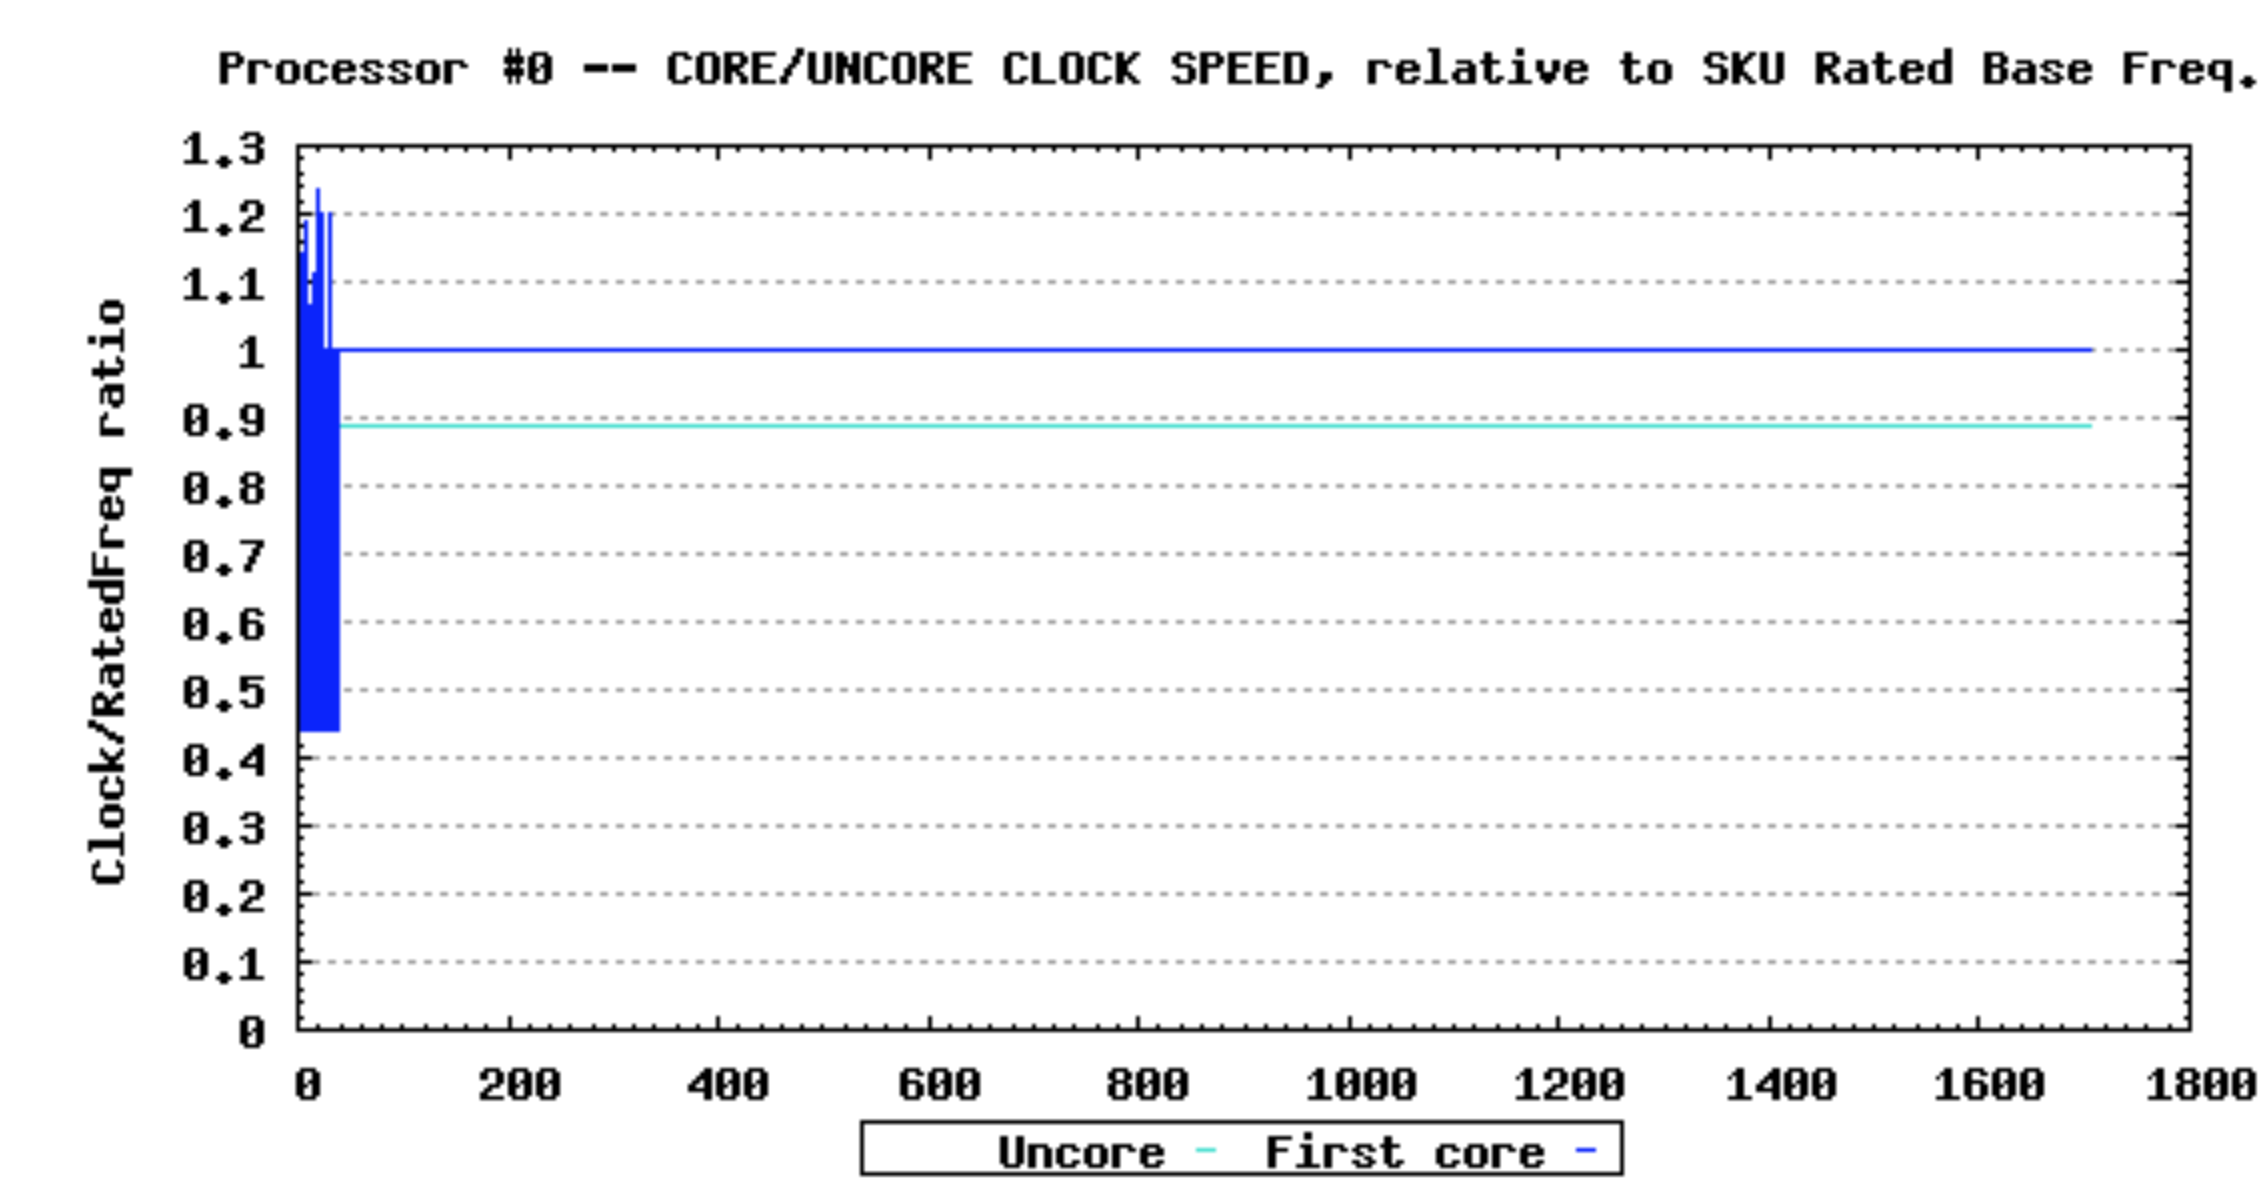
\includegraphics[width=\linewidth]{images/kg_freq.png}
            \caption{Évolution de la fréquence. Un ratio de 1 correspond à la fréquence de base de processeur (2.7 GHz).}
            \label{pic_kg_freq}
        \end{subfigure}
        ~ %add desired spacing between images, e. g. ~, \quad, \qquad, \hfill etc. 
          %(or a blank line to force the subfigure onto a new line)
        \begin{subfigure}[t]{0.45\linewidth}
            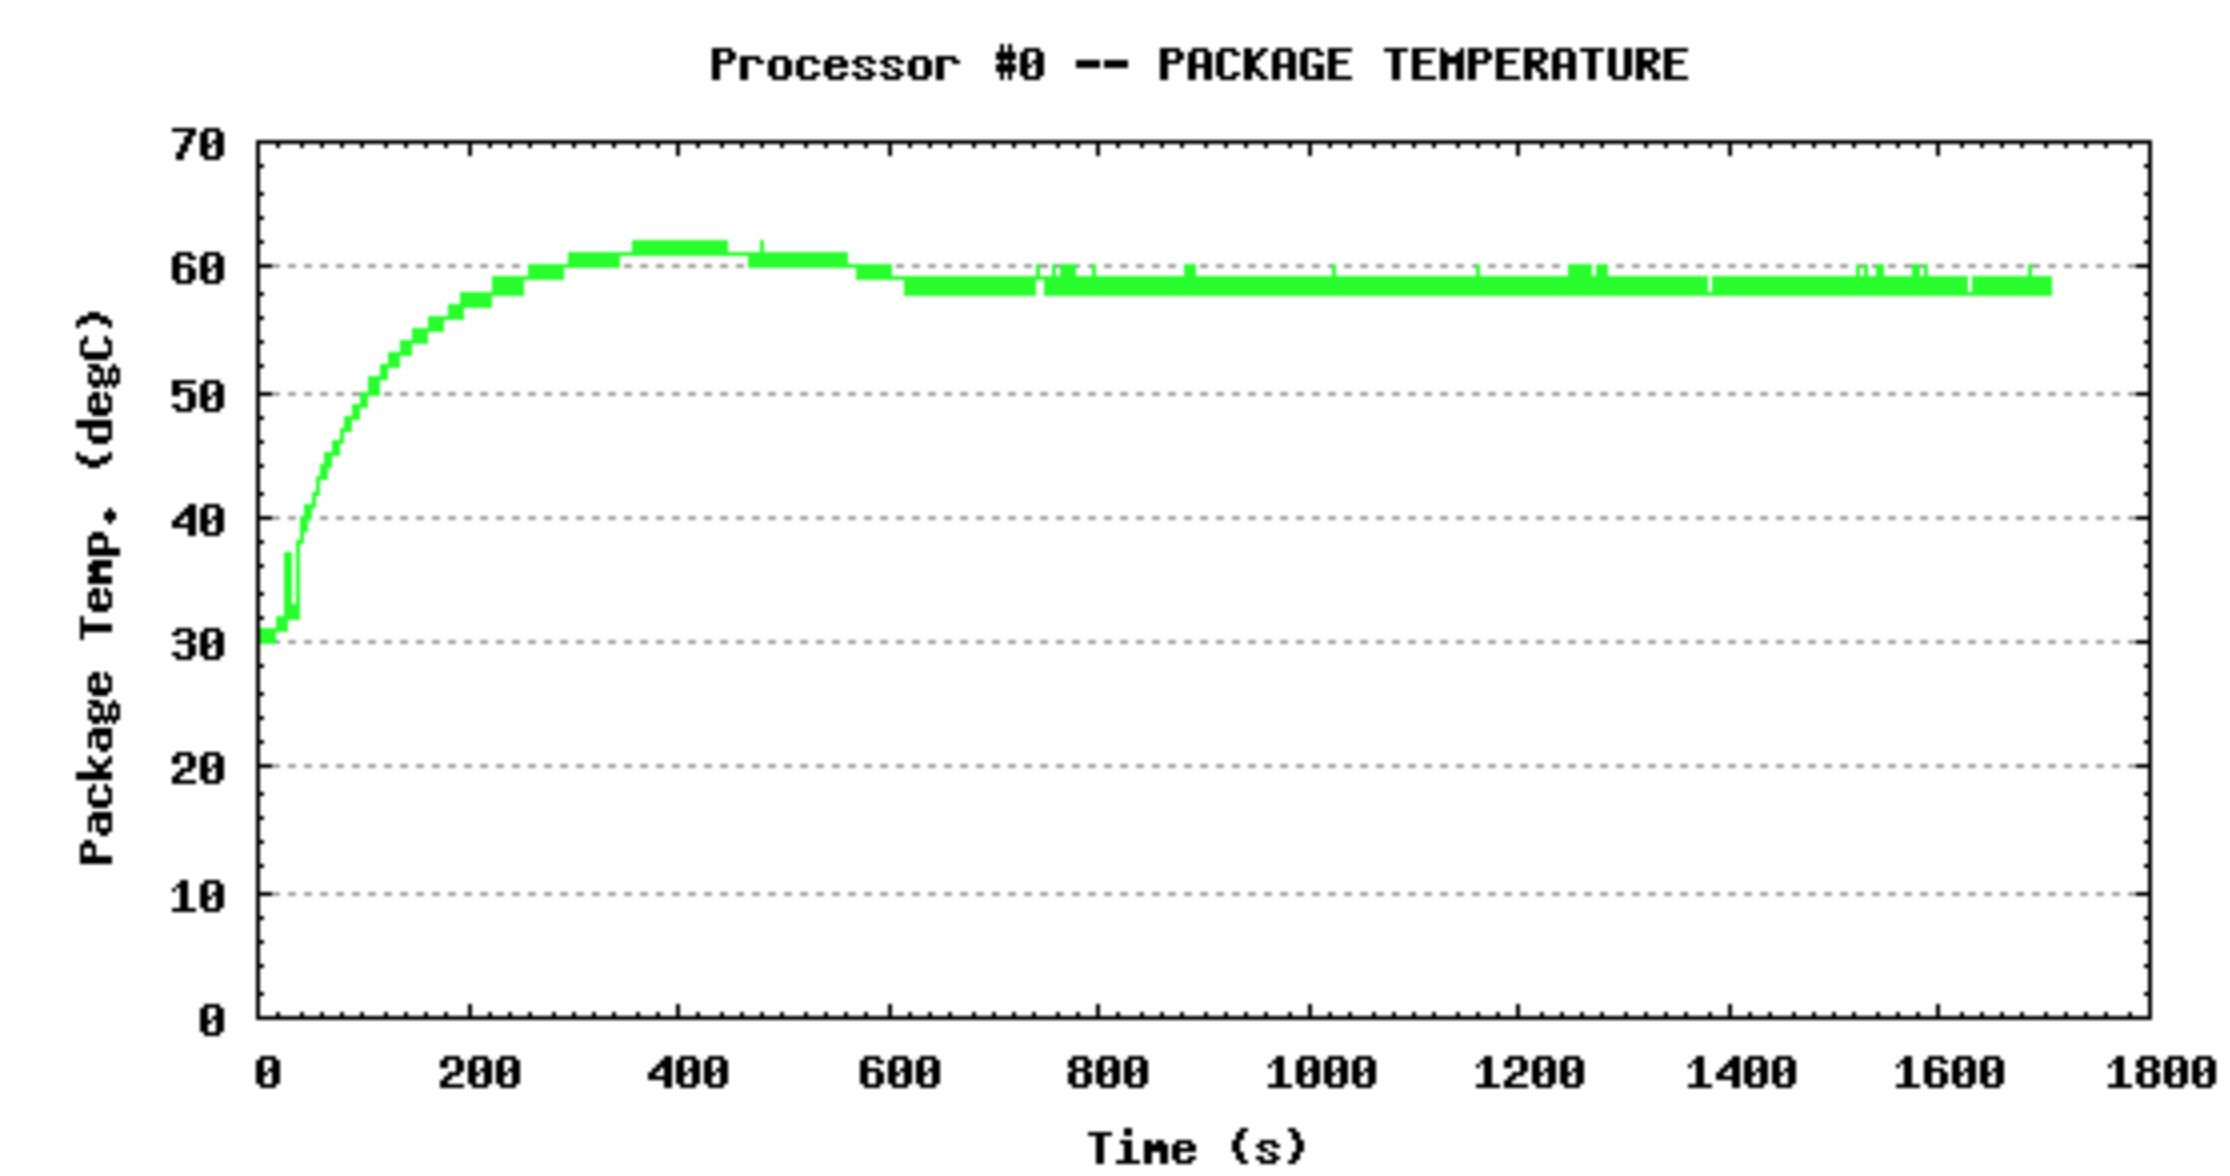
\includegraphics[width=\linewidth]{images/kg_temp.png}
            \caption{Évolution de la température du processeur}
            \label{pic_kg_temp}
        \end{subfigure}
        \caption{Évolution de la fréquence et de la température du processeur pour un benchmark AVX 2.0 exécuté sur 18 coeurs avec le turbo désactivé}\label{pic_kg_freq_vs_temp}
    \end{figure}
    \textbf{todo agrandir ou mettre l'un en dessus de lortre}

        




    
    \subsubsection{Caractérisation de la micro-architecture Haswell}
    %%%%%%%%%%%%%%%%%%%%%%%%%%%%%%%%%%%%%%%%%%%%%%%%%%%%%
    Lors de l'utilisation d'une nouvelle plateforme, l'utilisateur peut utiliser le \verb|Kernel Generator| pour caractériser la microarchitecture et trouver ses points forts ou points faibles. Lors de l'arrivée des processeurs Intel de génération Haswell en 2013, certains codes ont connu des baisses de performances malgré l'utilisation d'une architecture plus récente. Nous avons utilisé le \verb|Kernel Generator| pour caractériser les performances d'exécution des additions et des multiplications avec la commande suivante : \verb|./kg  -P double -W 64 -O mmmmm| permettant de générer le benchmark suivant:
    
    \begin{minipage}{0.97\linewidth}         \begin{lstlisting}[label=lst:kg_mul ,language=C]
for (i = 0; i < NB_lOOP; i++) {
timeStart = mygettime();
cycleInStart = rdtsc();
__asm__ ("" 
     "myBench:"  
   		"vmulsd %%xmm0, %%xmm1, %%xmm2; "
   		"vmulsd %%xmm0, %%xmm1, %%xmm3; "
   		"vmulsd %%xmm0, %%xmm1, %%xmm4; "
   		"vmulsd %%xmm0, %%xmm1, %%xmm5; "
   		"vmulsd %%xmm0, %%xmm1, %%xmm6; "
     "sub  $0x1, %%eax;"
     "jnz  myBench;"		:: "a" (NB_lOOP_IN));
cycleInEnd = rdtsc();
timeEnd = mygettime();
cycle_total += (cycleInEnd - cycleInStart);
time_total += timeEnd - timeStart;
}
\end{lstlisting} \end{minipage}
    
     La microarchitecture Haswell est capable d'exécuter deux multiplications par cycle. Cependant, l'utilisation du \verb|Kernel Generator| nous a montré que le processeur n'était pas capable d'exécuter des additions au même rythme que les multiplications. Les résultats présentés dans le \autoref{tab:mul_vs_add} montrent que la microarchitecture Haswell est capable d'exécuter deux multiplications contre une seule addition par cycle.

    \begin{table}[h!]
    \centering
    \begin{tabular}{|l|c|c|c|c|}
        \hline
        Opération & Nombre d'instructions & Frequence & Temps & IPC \\ \hline
        Multiplication & 40000000000 & 2.1 & 7.71 & \textbf{2} \\ \hline
        Addition & 40000000000 & 2.1 & 14.43 & {\color[HTML]{963400} \textbf{1}} \\ \hline
        \end{tabular}%
        
        \caption{Différence de performance lors de l'exécution d'addition et de multiplication sur une architecture Haswell.}
        \label{tab:mul_vs_add}
    \end{table}
    
    Bien sûr, cette caractéristique est documentée et en comptant le nombre de ports destinés aux additions, l'utilisateur du processeur aurait pu en trouver la raison. Cependant la lecture de la documentation de la microarchitecture dépasse le millier de pages et en comprendre les moindres détails est plus difficile que d'utiliser les bons outils. Nous pensons que le \verb|Kernel Generator| peut permettre à n'importe quel utilisateur de rapidement trouver ce genre de caractéristiques. Avant même d'avoir exécuté son application sur une nouvelle plateforme, il peut rapidement se faire une idée de ses performances et trouver ce genre de défauts.




    \subsubsection{Caractérisation de l'exécution dans le désordre}\label{sec:kg_out_of_order_dependency}
    %%%%%%%%%%%%%%%%%%%%%%%%%%%%%%%%%%%%%%%%%%%%%%%%%%%%%

    La puissance d'un supercalculateur vient de sa capacité à réaliser des calculs en parallèle. Pour satisfaire la loi d'Amdahl (voir \autoref{sec:amdhal}). La tâche des développeurs est de maximiser les zones de codes pouvant profiter des ressources parallèles des architectures. Le principal frein à l'utilisation du parallélisme vient de zones de codes dites séquentielles dont les instructions doivent être exécutées à la suite les unes des autres. Cela peut être dû à la dépendance d'une instruction au résultat de l'instruction précédente. Les performances d'un tel code sont souvent très mauvaises car une seule ressource de calcul (un coeur) peut être utilisée pour leur exécution. Cependant, la nature des algorithmes peut assez fréquemment laisser place à certaines optimisations. Dans le domaine des finances, les algorithmes de Monte-Carlo sont très utilisés. Ces codes ont la particularité d'exposer de longues chaînes de dépendances. En restructurant le code, le programmeur peut espérer profiter de l'exécution dans le désordre (voir \aref{sec:out_of_order}). Cela nécessite cependant d'apporter suffisamment d'instructions indépendantes au processeur pour qu'il puisse les exécuter en parallèle. Le processeur est capable d'exécuter plusieurs chaînes indépendantes les unes des autres. La performance d'une telle plateforme dépend alors de sa capacité à en exécuter plusieurs en parallèle. Grâce à l'option \verb|--dependency N| du \verb|Kernel Generator|, le benchmark peut être utilisé pour caractériser cette fonctionnalité matérielle en générant $N$ chaînes indépendantes. En utilisant une dépendance de 1, chaque instruction a besoin du résultat de l'instruction précédente (voir \autoref{lst_dep1}). Dans ce cas-là, aucune parallélisation n'est possible pour le processeur. L'exécution de ce code atteint un \gls{IPC} de 0.25. Le processeur a besoin de 4 cycles d'horloge pour exécuter une instruction. Le faible IPC vient de la nécessité d'attendre que le résultat de l'opération précédente soit disponible pour pouvoir commencer à être exécutée. Sur le processeur utilisé, l'exécution d'une multiplication AVX-512 est de 4 cycles.
    
    
    
    
\begin{minipage}{0.97\linewidth}         \begin{lstlisting}[label=lst_dep1,language=C, caption=Code généré par la commande \texttt{/kg -W 512 -P double -O mmmmm -D 1}. Chaque instruction utilise le résultat produit par l'instruction précédente.]
"myBench: " 
	"vmulpd %%zmm0, %%zmm6, %%zmm2; "
	"vmulpd %%zmm0, %%zmm2, %%zmm3; "
	"vmulpd %%zmm0, %%zmm3, %%zmm4; "
	"vmulpd %%zmm0, %%zmm4, %%zmm5; "
	"vmulpd %%zmm0, %%zmm5, %%zmm6; "
"sub  $0x1, %%eax;"
"jnz  myBench;"
\end{lstlisting} \end{minipage}

     
    Pour évaluer la capacité du processeur à exécuter plusieurs chaînes indépendantes, différents nombres de chaînes ont pu être générées grâce à l'option \verb|--dependecy N|. Le code généré pour 4 chaînes est présenté sur la \autoref{pic_kg_dep_4}. En faisant varier le nombre de chaînes indépendantes, les résultats présentés dans le \autoref{tab_kg_depth} ont été obtenus. Grâce au tampon d'instructions de système d'exécution dans le désordre, le processeur est capable de commencer l'exécution de plusieurs chaînes indépendantes simultanément. Nous avons pu valider que le processeur est capable d'exécuter au moins 8 chaînes d'instructions indépendantes. Le processeur peut exécuter une multiplication par cycle par pipeline (2 au total). La latence d'une multiplication AVX-512 étant de 4 cycles, le processeur a besoin de 8 chaînes indépendantes pour utiliser la totalité de la puissance du processeur. Cette caractéristique du processeur doit être connue par le programmeur pour transformer son code et obtenir le maximum de performance du processeur. Grâce au \verb|Kernel Generator|, les nouvelles architectures peuvent être testées pour caractériser ces performances et prévoir leur performance pour des codes pouvant utiliser des chaînes de calculs indépendantes comme la résolution de polynômes par exemple. 
    
         \begin{figure}
            \center
            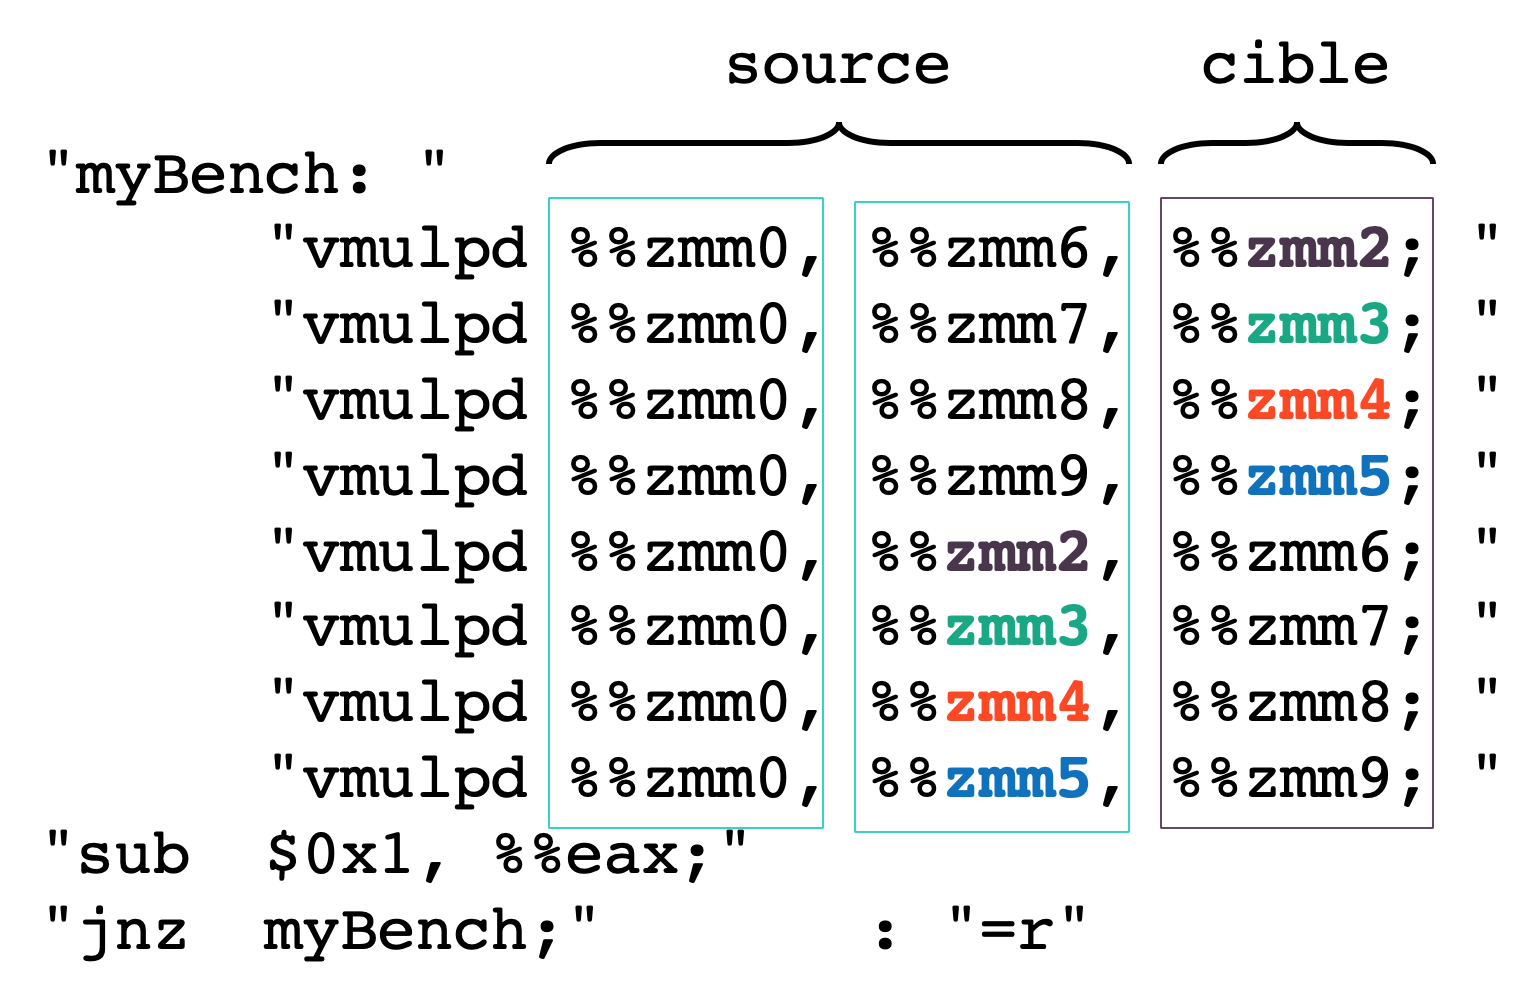
\includegraphics[width=8cm]{images/kg_dep_4.png}
            \caption{\label{pic_kg_dep_4} Code généré par la commande \texttt{/kg -W 512 -P double -O mmmmmmmm -D 4}. Les quatre chaînes de dépendance sont représentées par les quatre couleurs utilisées.}
        \end{figure}

    \begin{table}[h!]
    \centering
    \normalsize
    \begin{tabular}{|l|c|c|c|c|c|c|c|c|c|c|}
    \hline
    Nombre de chaînes & 1 & 2 & 3 & 4 & 5 & 6 & 7 & 8 & 9 & 10 \\ \hline
    IPC & 0.25 & 0.50 & 0.75 & 1 & 1.25 & 1.50 & 1.75 & 2 & 2 & 2 \\ \hline
    \end{tabular}%
    \caption{Mesure du nombre d'instruction par cycle pour un nombre de chaîne de dépendance $N$, dans un benchmark généré à l'aide de la commande \texttt{/kg -W 512 -P double -O mmmmmmmm -D N}. Au moins 8 chaînes d'instructions indépendantes doivent être présentées au processeur pour l'utiliser au maximum de ses performances (IPC égal à 2).}
    \label{tab_kg_depth}
    \end{table}





    \subsubsection{Caractérisation de la FPU de deux processeurs Skylake}

        La dernière génération de processeur Intel Skylake est répartie en quatre gammes (Bronze, Silver, Gold et Platinium). Les fonctionnalités et les performances des processeurs des différentes gammes étant différentes (voir \autoref{table:skl}), il est important pour notre équipe avant-vente d'en connaître les caractéristiques et les performances pour adapter les configurations des serveurs aux demandes des clients. Les processeurs des gammes Bronze ou Silver sont rarement choisis pour répondre à un appel d'offres compte tenu de leurs caractéristiques plus faibles (une FPU au lieu de deux, nombre plus faible de coeurs). Les processeurs haut de gamme (Gold et Platinium) possèdent généralement plus de coeurs, et sont capables d'utiliser des fréquences plus élevées que les processeurs d'entrée de gamme (Bronze et Silver). Bien sûr, comme ces processeurs coûtent plus cher à l'achat, un client choisira un processeur en fonction de son budget, de sa consommation électrique ou du profil de son application.
        
        
        \begin{table}[h!]
        \centering
        \resizebox{\textwidth}{!}{%
        \begin{tabular}{|l|l|l|l|l|l|}
        \hline
        \rowcolor[HTML]{EFEFEF}
        Gamme - référence CPU                                &   Bronze: 31xx                    & Silver: 41xx              & Gold: 51xx            & Gold: 61xx            & Platinium: 81xx           \\ \hline
        Nb. canaux mémoire et vitesse    & 6-ch@2133 Ghz                         & 6-ch\textbf{@2400}      & 6-ch@2400           & 6-ch\textbf{@2666}   & 6-ch@2666                \\ \hline
        Lien UPI (scalabilité)         &     2   (2S-2UPI)       & 2  (2S-2UPI)    & 2 (4S-2UPI)  & 3  (2S-3UPI) & 3    (8S-3UPI)    \\ \hline
        Débit UPI                   & 9.6 GT/s                          & 9.6 GT/s                  & 10.4 GT/s              & 10.4 GT/s             & 10.4 GT/s                 \\ \hline
        HyperThreading  \cite{Marr2002}                &   NON                              & \textbf{OUI}              & OUI                   & OUI                   & OUI                       \\ \hline
        FMA-512 FPU                     &     1                             & 1                         & 1                     & \textbf{2 }           & 2                         \\ \hline
        
        \end{tabular}
        }
        \caption{Principales différences entre les gammes de processeurs Intel de génération Skylake.}
        \label{table:skl}
        
        \end{table}
        
      
      Pour caractériser la performance crête des processeurs \gls{flopsmax}, notre équipe de benchmark utilise des codes tels que HPL. Pour obtenir la meilleure performance atteignable, le benchmark HPL est compilé pour utiliser les instructions vectorielles les plus grandes supportées par le processeur étudié (ici des instructions AVX-512). Les résultats du benchmark Linpack donnés dans le \autoref{table:skl_bench}, montrent que les processeurs les plus performants sont ceux appartenant aux gammes Gold et Platinium. Cette différence de performance peut être expliquée par la présence de deux \gls{FPU} sur les processeurs haut de gamme. Ces deux FPU sont capables d'exécuter chacune une instruction \gls{FMA} AVX-512 par cycle. Grâce au \verb|Kernel Generator|, cette caractéristique a pu être vérifiée (voir \autoref{table:skl_bench}). 

        \begin{table}[h!]
        \centering
        
        \resizebox{\textwidth}{!}{%
        \begin{tabular}{|l|l|l|l|l|}
        \hline
        \rowcolor[HTML]{EFEFEF}
        Processeur (Nb. FPU)    & Silver: 4110 (1)  & Gold: 5117 (1)   & Gold: 6130 (2)    & Platinium: 8160 (2)        \\ \hline
        Instruction AVX-512 FMA par cycle   & 1             & 1            & 2             & 2                    \\ \hline
        Benchmark HPL (GFLOPS)            & 297           & 372          & 714           & 716                  \\ \hline
        
        \end{tabular}
        }
        \caption{Pour différents processeurs, le nombre d'instructions FMA AVX-512 pouvant être exécutée chaque cycle a été mesuré à l'aide du \texttt{Kernel Generator}. En fonction du nombre de FPU présent sur un coeur (1 ou 2), le nombre d'instructions exécutées varie (1 ou 2). La performance \gls{flopsmax} du benchmark HPL mesurée GFLOPS varie de la même façon suivant la gamme du processeur utilisé. Afin de pouvoir comparer les différentes gammes de processeurs, la configuration suivante a été appliquée à chaque processeur: désactivation de l'\textit{hyperthreading}, fréquence limitée à 1.5 GHz, utilisation de 8 coeurs. \textbf{todo: revoir les valeurs}}
        \label{table:skl_bench}
        \end{table}
        % 1 FPU : 8 * 2 *1 *1.5 * 8 = 192
        % 2 FPU : 8 * 2 *2 *1.5 * 8 = 384
        
        
        Afin d'estimer l'impact d'une FPU manquante sur la performance d'une application réelle, nous avons utilisé une application de CFD\textbf{todo C KOI ?} typique. L'application utilisée n'exécute que des instructions vectorielles de 256 bits (AVX-2). Nous nous attendons alors à obtenir des performances différentes entre un processeur de gamme Silver et de gamme Gold pour une application qui n'est pas limitée par la bande passante mémoire. Étonnamment, les résultats obtenus sur ces deux plateformes sont très proches. Pourtant, nous avons bien montré que les processeurs de gamme supérieure possèdent une FPU de plus et sont donc deux fois plus performants. Pour comprendre ce phénomène, nous avons utilisé le \verb|Kernel Generator| pour générer un kernel de calculs utilisant des instructions vectorielles de 256 bits. La performance mesurée pour le kernel est reportée dans le \autoref{table:skl_bench2}.  
        
       
        
        
        \begin{table}[h!]
        \centering
        % increase table row spacing, adjust to taste
        %\renewcommand{\arraystretch}{1.1}
        % COMMENTS if using array.sty, it might be a good idea to tweak the value of
        %\extrarowheight{1} as needed to properly center the text within the cells

        \resizebox{0.4\textwidth}{!}{%
        \begin{tabular}{|l|l|l|l|l|}
        \hline
        \rowcolor[HTML]{EFEFEF}
                                & Silver: 4110       & Gold: 6130      \\ \hline
        IPC                     & 2                  & 2           \\ \hline
        GFLOP/s                 & 2.38e+10           & 2.37e+10           \\ \hline
        \end{tabular}
        }
        \caption{Mesure de la performance de processeur de deux gammes différentes à l'aide du \texttt{Kernel Generator} et de la commande suivante: \texttt{/kg  -P double -W 256 -O ffffffff}. Alors que le processeur de la gamme Gold possède une FPU de plus, il obtient des performances similaires à celles du processeur de gamme Silver.}
        \label{table:skl_bench2}
        \end{table}
        
        Bien que le processeur Intel Xeon Silver 4110 ne possède qu'une seule \gls{FPU}, il est capable d'exécuter deux instructions AVX-2 par cycle. Cette caractéristique peut être retrouvée dans la documentation du processeur \footnote{source: \url{https://en.wikichip.org/wiki/intel/microarchitectures/skylake\#Execution_engine_2}}. Les FPU des processeurs Skylake d'entrée de gamme fusionnent deux ports de 256 bits pour former la FPU 512-bits. Cependant, lorsque des instructions de 256 bits sont exécutées, le processeur peut utiliser les deux ports indépendamment pour exécuter deux instructions de 256 bits. La FPU supplémentaire présente sur les processeurs haut de gamme est une FPU 512 bits qui ne permet pas d'utiliser cette caractéristique et qui pourrait permettre d'exécuter (en théorie) quatre instructions par cycle.
        Afin de mieux comprendre comment cette fusion d'instructions fonctionnait, nous avons utilisé le \verb|Kernel Generator| pour générer des \glspl{kernel} possédant des instructions vectorielles de taille différentes. Les résultats des différentes expérimentations sont reportés dans le \autoref{res:skl}. Chaque cycle, la FPU est capable d'exécuter différentes combinaisons d'instructions: 


        \begin{itemize}
            \item Une instruction AVX 512 bits,
            \item Deux instructions AVX 256 bits,
            \item Deux instructions AVX 128 bits,
            \item Deux instructions scalaires,
            \item Toute combinaison de deux instructions dont la taille agrégée ne dépasse pas 512 bits.
        \end{itemize}
        
        
        \begin{table}[h!]
        \normalsize
        % increase table row spacing, adjust to taste
        %\renewcommand{\arraystretch}{1.1}
        % COMMENTS if using array.sty, it might be a good idea to tweak the value of
        %\extrarowheight{1} as needed to properly center the text within the cells
        \centering
        %\resizebox{\textwidth}{!}{%
        \begin{tabular}{|l|c|c|c|c|}
            \hline
            \rowcolor[HTML]{EFEFEF} 
            Gamme & Silver & Gold & Gold & Platinium \\ \hline
            \rowcolor[HTML]{EFEFEF} 
            Ref. processeur Intel Skylake & 4110 & 5117 & 6130 & 8160 \\ \hline
            \rowcolor[HTML]{EFEFEF} 
            Nombre de FPU & 1 & 1 & 2 & 2 \\ \hline
            128 + scalaire & \textbf{2} & \textbf{2} & 2 & 2 \\ \hline
            256 + scalaire & \textbf{2} & \textbf{2} & 2 & 2 \\ \hline
            256 + 128 & \textbf{2} & \textbf{2} & 2 & 2 \\ \hline
            256 & \textbf{2} & \textbf{2} & 2 & 2 \\ \hline
            512 + scalaire & 1 & 1 & 2 & 2 \\ \hline
            512 + 128 & 1 & 1 & 2 & 2 \\ \hline
            512 + 256 & 1 & 1 & 2 & 2 \\ \hline
        
        \end{tabular}
        %}
        \caption{Mesure du nombre d'instruction exécutées chaque cycle pour différents processeurs. La FPU des processeurs d'entrée de gamme est capable de fusionner certaines instructions (en gras) pour les exécuter en un seul cycle.}
        \label{res:skl}
        \end{table}
        
        
        
       Ainsi, le processeur haut de gamme bénéficie des deux FPU lorsque le code est capable d'utiliser des instructions vectorielles de 512 bits. Il est fréquent que les applications n'y parviennent pas (mauvaise vectorisation du code, problème du compilateur, dépendances) et utilisent des instructions vectorielles plus petites. Les processeurs d'entrée de gamme obtiennent alors des performances rigoureusement égales. Évidement, la FPU n'est pas la seule responsable de la performance d'une application, le \autoref{table:skl} montre bien que d'autres caractéristiques diffèrent telles que le nombre de liens UPI ou la possibilité d'utiliser l'hyperthreading. Le but du \verb|Kernel Generator| est de caractériser une architecture pour le besoin d'une application. Grâce aux caractéristiques découvertes suite à cette expérimentation, plusieurs réponses à des offres d'appels ont été réalisées avec des processeurs d'entrée de gamme. Grâce à cette caractéristique, les applications utilisant des instructions AVX-2 peuvent obtenir des performances assez proches sur des processeurs coûtant beaucoup moins cher.


        
        




%    \subsubsection{Expliquer les performances d'un code}
    %%%%%%%%%%%%%%%%%%%%%%%%%%%%%%%%%%%%%%%%%%%%%%%%%%%%%
 %   Une autre utilisation du \verb|Kernel Generator| peut permettre d'expliquer les performances d'une autre application. 
    
    
  %   What we have seen in the past months with the releases of the new Skylake processors is that entry level processors like Intel 4110 can perform as good as a top bin processor like the Intel 6148 for real applications thus increasing the $\frac{performance}{price}$ of a large scale cluster. 


\subsection{Conclusion}
%%%%%%%%%%%%%%%%%%%%%%%%%%%%%%%%%%%%%%%%%%%%%%%%%%%%%
    
    L'outil \verb=Kernel Generator= est un \verb|Kernel Generator| qui permet de mesurer la performance maximale (\gls{flopsmax})  d'un processeur pour un type d'instruction vectorielle utilisant différentes configurations (type d'instructions, dépendances...).
    Le \verb|Kernel Generator| assembleur est un outil très précis pour la caractérisation des \gls{FPU}. Le principal avantage de l'utilisation de l'assembleur est d'éliminer les optimisations du compilateur. Le benchmark doit assurer à l'utilisateur qu'il mesure bien la performance du code qu'il a choisi de générer et qu'il n'a pas été modifié durant la compilation. Il nous a permis d'atteindre des performances souvent égales aux performances théoriques (\gls{flopspeak}). En utilisant le générateur, le programmeur peut être amené à découvrir des particularités de la microarchitecture (comme celle de l'exécution dans le désordre). En comprenant précisément le fonctionnement de la FPU, il pourra même trouver des optimisations pour sa propre application.
    
    Pour le moment, seul l'ISA x86 est supporté, mais l'outil a été codé de façon à faciliter l'ajout d'une nouvelle ISA. Nous avons choisi de commencer à le développer pour des processeurs dont nous connaissons bien le comportement pour valider son bon fonctionnement. L'exemple de la FPU du processeur Intel Xeon 4110, nous a permis de montrer que même sur des architectures que nous connaissons bien, certaines spécificités nous échappent encore. L'utilisation du générateur permet d'en comprendre toutes les particularités.
    
    
    \paragraph{Perspectives} La suite du travail comprend la fin du développement de l'option permettant de mélanger différentes tailles d'instructions vectorielles dans le même kernel. Nous souhaitons développer une option qui permettra de générer des instructions \textbf{TODO verbe pour remplacer générer} des déplacements mémoires afin vérifier qu'elles ne gênent pas l'exécution des instructions de calcul. Enfin, pour mieux caractériser les plateformes pour certaines applications comme en cryptographie, nous allons ajouter d'autres instructions pouvant être générées (rotation, décalage...). \textbf{todo reprendre}
    
    